%%%%%%%%%%%%%%%%%%%%%%%%%%%%%%%%%%%%%%%%%%%%%%%%%%%%%%%%%%%%%%%%%%%%%%%%%%%%


\documentclass[draft]{agujournal2019}
\usepackage{url} 
%\usepackage{lineno}
%\usepackage[inline]{trackchanges} %for better track changes. finalnew option will compile document with changes incorporated.
\usepackage{soul}
\usepackage{lscape}
\usepackage{adjustbox}
\usepackage{float}
\usepackage{amsmath}
\usepackage{amssymb}
\usepackage{amsthm}
\usepackage{physics}
\usepackage{setspace}
\usepackage{fix-cm}
\usepackage{booktabs}

\usepackage{subcaption}

\usepackage{graphicx}

\usepackage{wrapfig}
\usepackage{blindtext}
%Table-related commands
\usepackage{array}
%\setlength{\arrayrulewidth}{1mm}
%\setlength{\tabcolsep}{18pt}
%\renewcommand{\arraystretch}{1.5}
%\newcolumntype{s}{>{\columncolor[HTML]{AAACED}} p{3cm}}
% %-------------------------------------------------------


% defined commands
\newcommand{\unit}[1]{\ensuremath{\, \mathrm{#1}}}
% "Colored Marker" commands: wrap text in, e.g., \red{...} to highlight that color
\newcommand{\red}[1]{\textcolor{red}{#1}}
\newcommand{\blue}[1]{\textcolor{blue}{#1}}
\newcommand{\purple}[1]{\textcolor{purple}{#1}}
\newcommand{\avg}[1]{\left\langle #1 \right\rangle}
\newcommand{\vel}[0]{\mathbf{u}}
\newcommand{\B}[0]{\mathbf{B}}

%uncomment this for single-spaced version
\draftfalse

\begin{document}
\SetSinglespace{}
% preliminary title
\title{[PHYS 6268] Nonlinear Dynamics: Problem Set 4}

% I defaulted to alphabetical last name, no preference here
\authors{C. Michael Haynes\affil{1}}

\affiliation{1}{School of Earth and Atmospheric Sciences, Georgia Institute of Technology, Atlanta GA, USA}


\section*{Strogatz Book: Problems 3.6.7, 3.7.6, 4.1.8, 4.2.2, 4.3.6, 4.4.1, \& 4.5.1}


\section{Problem 3.6.7: Simple model of a magnet}
\label{sec:p1}

A magnet can be modeled as an enormous collection of electron spins. In the simplest model (the Ising model), the spins can point only up or down, and are assigned the values $S_i=\pm1$ for $i\in\{
1,\dots,N\gg1\}$. For quantum mechanical reasons, the spins like to point in the same direction as their neighbors; on the other hand, the randomizing effects of the temperature tend to disrupt any such alignment. An import macroscopic property of the magnet is its average spin or \emph{magnetization}
\begin{equation*}
    m = \left|\frac{1}{N}\sum_{i=1}^N S_i \right|  \quad .
\end{equation*}
At high temperature, the spin points in random directions and so $m\approx0$; the material is in the paramagnetic state. As the temperature is lowered, $m$ remains near zero until a critical temperature $T_c$ is reached. Then a \emph{phase transition} occurs and the material spontaneously magnetizes. Now $m>0$, and we have a \emph{ferromagnet}. 
\par
The symmetry between up and down spins means that there are \emph{two} possible ferromagnetic states. This symmetry can be broken by applying an external magnetic field $h$, which favors either the up or down direction. Then, in an approximation called mean-field theory, the equation governing the equilibrium value of $m$ is 
\begin{equation*}
    h = T\tanh^{-1}{m} - Jnm \qquad ,
\end{equation*}
where $J$ and $n$ are constants; $J>0$ is the ferromagnetic coupling strength and $n$ is the number of neighbors of each spin.

\subsection{(a) Analyze the solutions $m^*$ of $h=T\tanh^{-1}{m} - Jnm$, using a graphical approach}
\label{ssec:p1a}
\par
\begin{figure}[h]
    \centering
    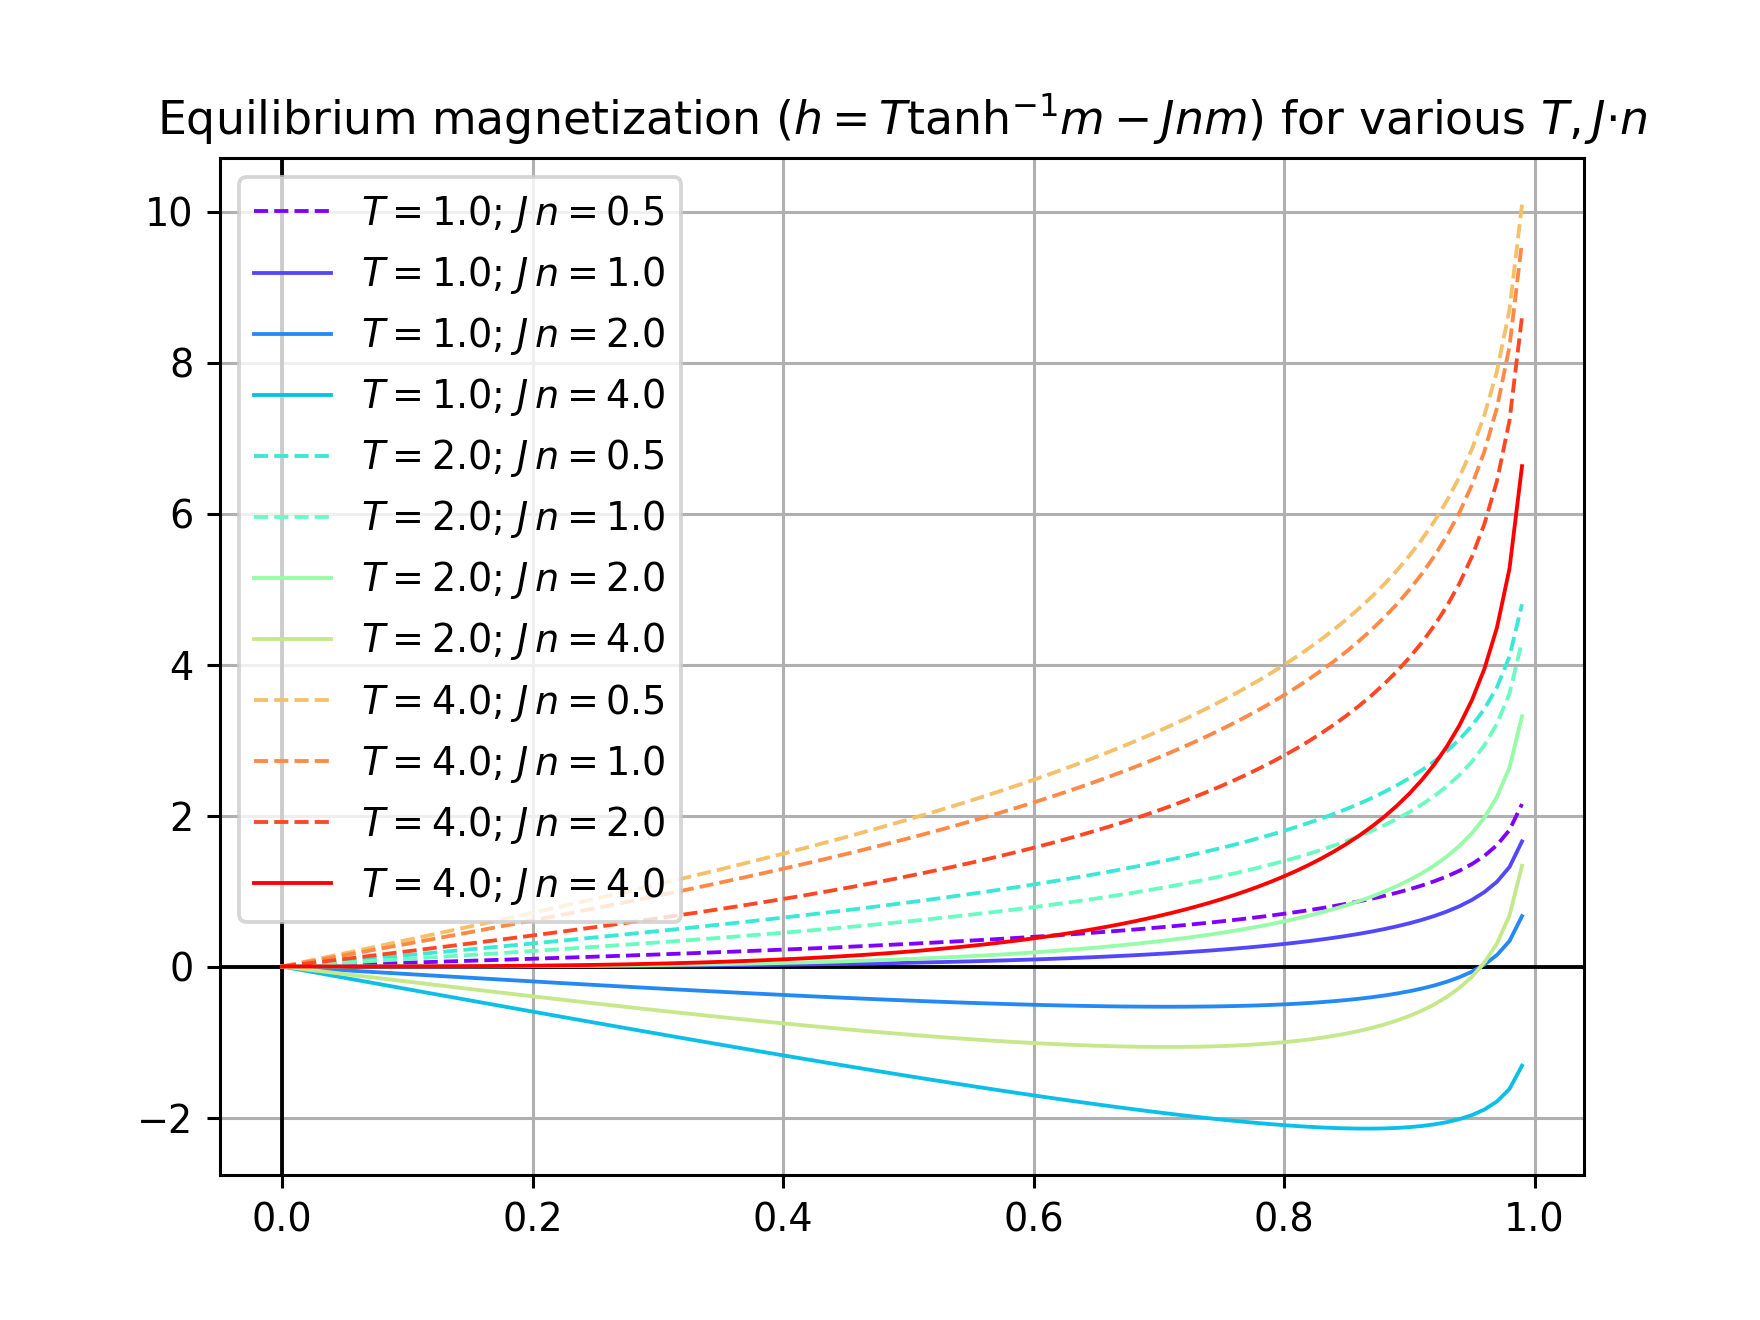
\includegraphics[width=0.8\linewidth]{figs/3.6.7_params.png}
    \caption{\scriptsize{Parameter survey for the expression for equilibria $m^*$, given by $h=T\tanh^{-1}{m} - Jnm$. The parameters $T>0$ and the product of $Jn>0$ are varied over a range to illustrate the behavior of this expression. Dashed curves indicate those with only a single equilibrium at $m^*=0$. }}
    \label{fig:p1_param}
\end{figure}
To analyze the equilibrium solutions $m^*$ of the above equation, we calculate $h(m)$ for several combinations of $T_c$ and $Jn$. Because $J$ and $n$ are both positive, their product is always greater than or equal to zero. Moreover, since these quantities only appear in the governing equation as factors of the same term, it is sufficient to vary the \emph{product} of $Jn>0$ as a single parameter. Figure \ref{fig:p1_param} shows various solutions $m^*$ of the expression $h=T\tanh^{-1}{m} - Jnm$. The color of the curve is labeled according to the parameters used to generate it. By inspection of the curves, the equilibria $m^*$ bifurcate when $T=Jn$. Solid curves indicate those that have multiple solutions of $m^*$: note that this includes curves with a double root at $m^*=0$, which occurs at the moment when $T=Jn$. Dashed curves indicate when the system only has a single, trivial equilibrium at $m^*=0$. 
\par
\begin{figure}[!h]
    \centering
    \begin{subfigure}[t]{0.45\textwidth}
        \centering
        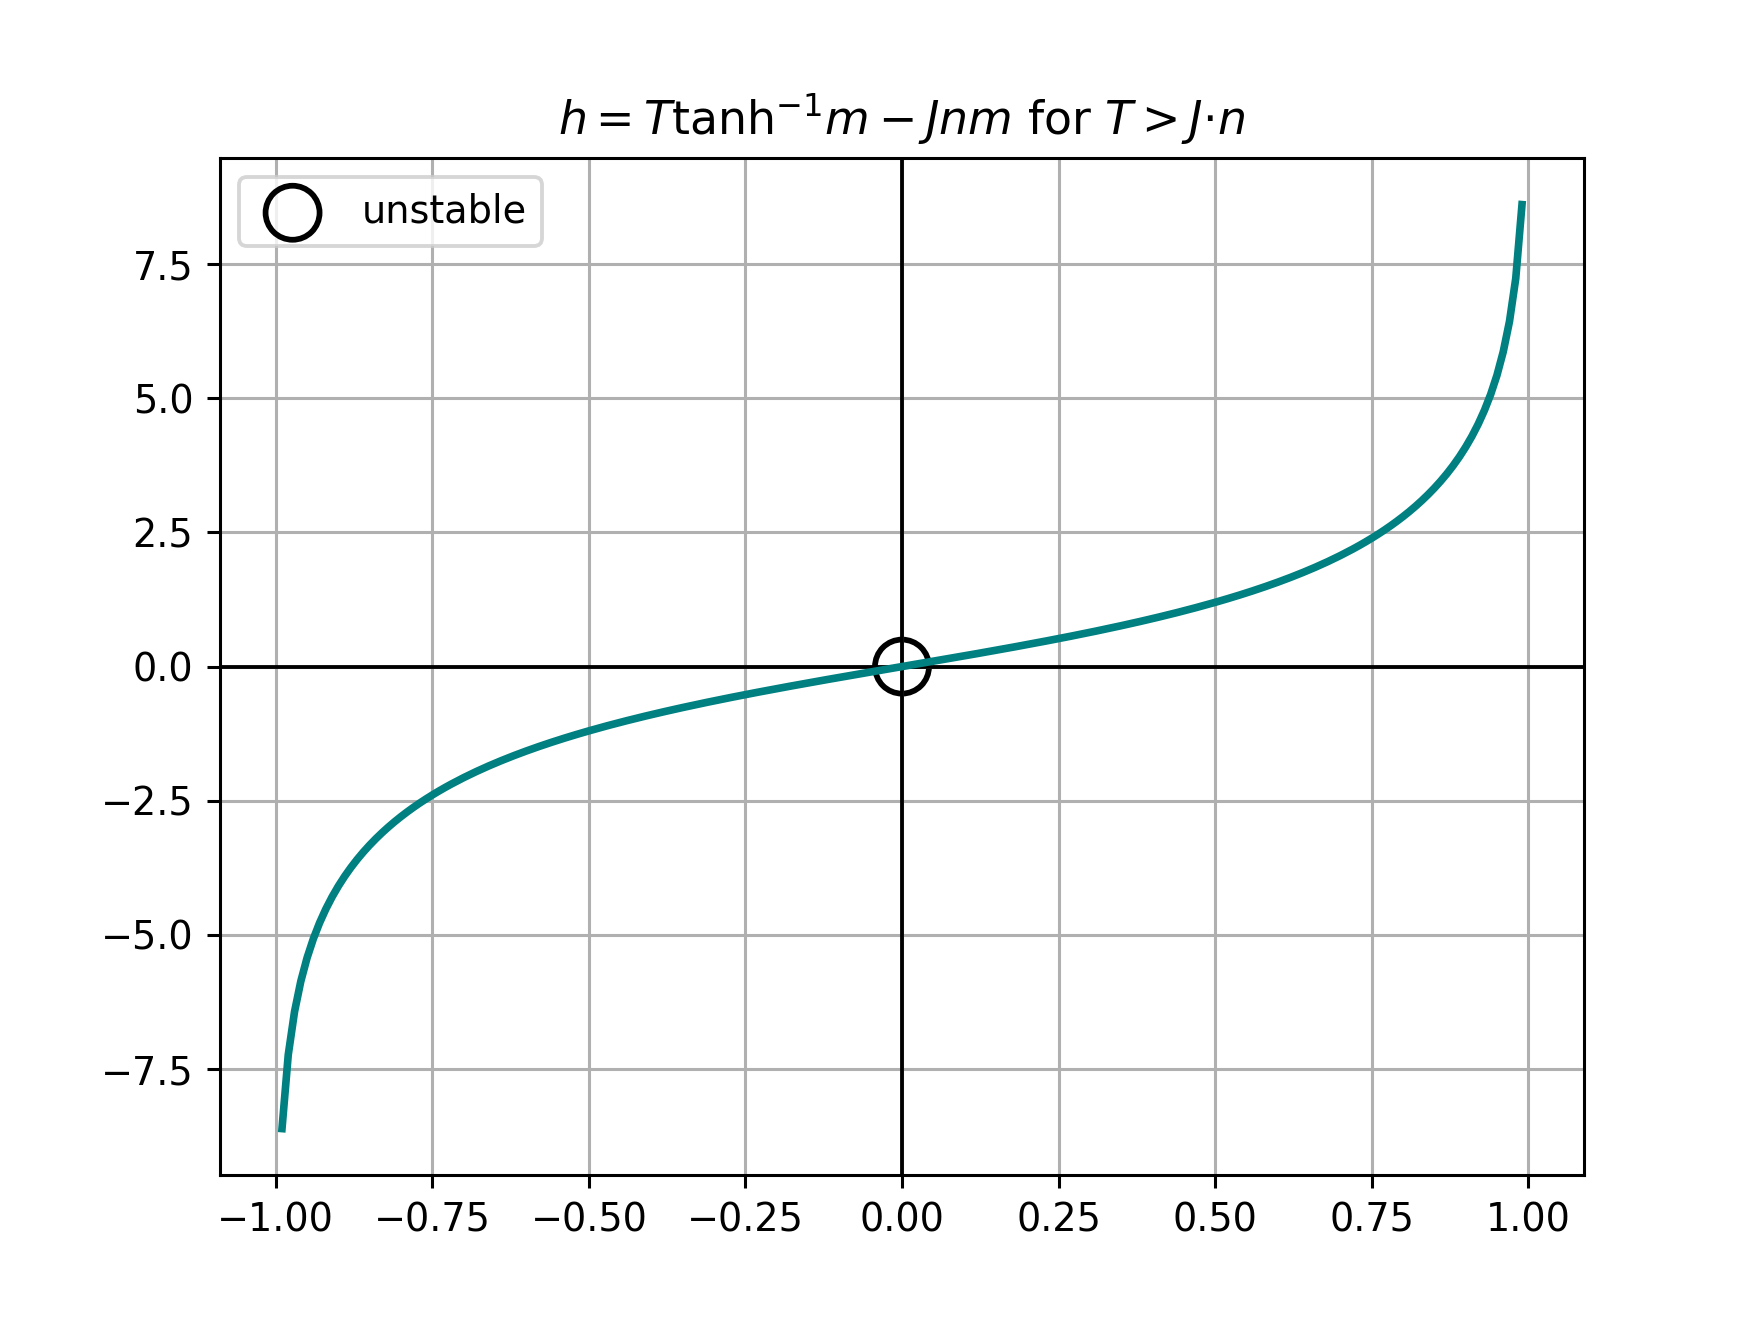
\includegraphics[width=\linewidth]{figs/3.6.7_Tg.png}
    \end{subfigure}
    \hfill
    \begin{subfigure}[t]{0.45\textwidth}
        \centering
        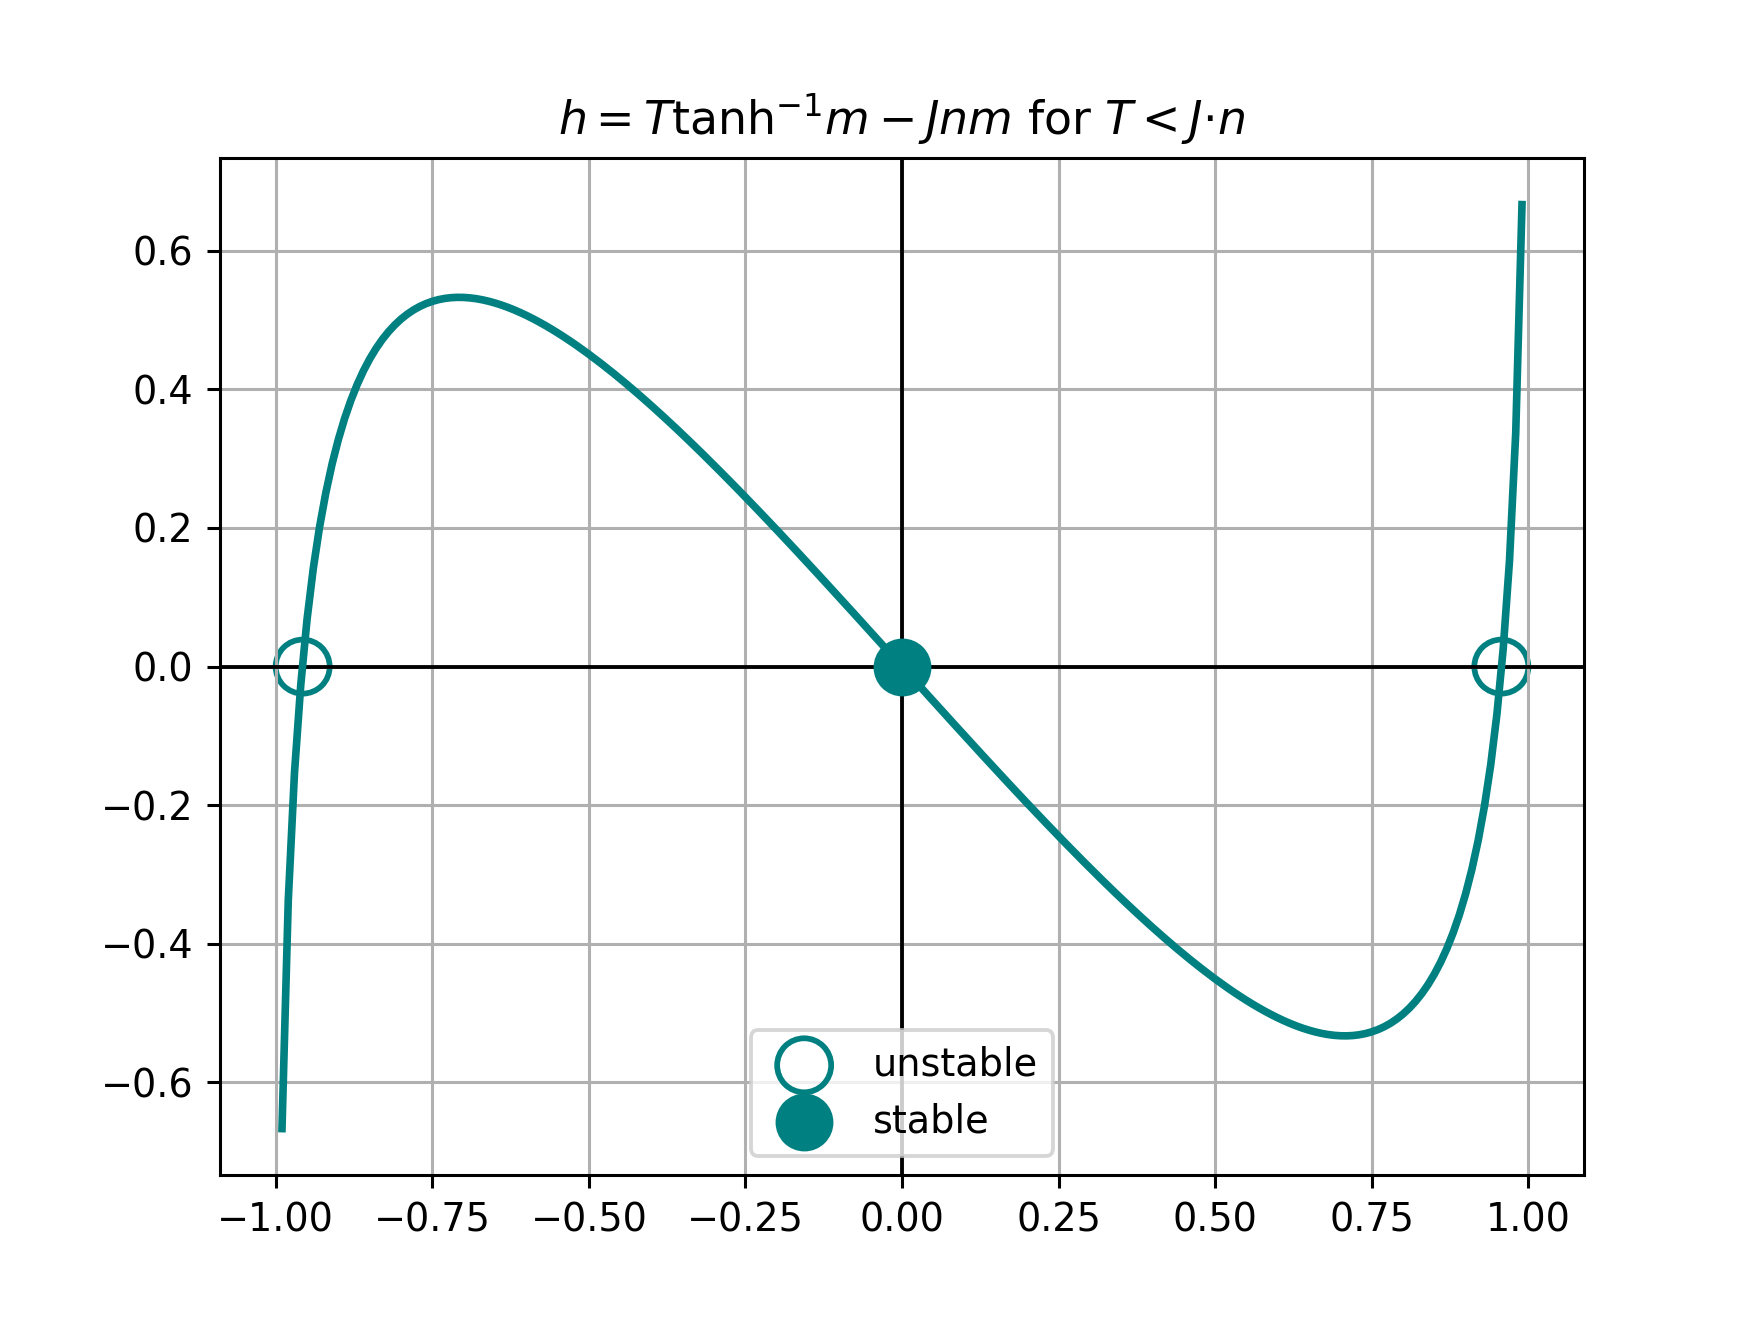
\includegraphics[width=\linewidth]{figs/3.6.7_Tl.png}
    \end{subfigure}
    \caption{\scriptsize{Examples depicting the equilibrium relationship for $m^*$ under the conditions $T>Jn$ (left) and $T<Jn$ (right). These systems support one unstable fixed point and one stable plus two unstable fixed points, respectively. }}
    \label{fig:p1_spef}
\end{figure}
To further illustrate the behavior of this system, we depict two more examples of the curve $h=T\tanh^{-1}{m} - Jnm$ on their own for clarity in Figure \ref{fig:p1_spef}. These exemplify the behavior of the expression for $m^*$ as $T$ transitions from above to below the $T_c$ threshold. As can be seen by comparing the left and right panels of Figure \ref{fig:p1_spef}, the bifurcation that occurs when $T=T_c$ involves a lone trivial and unstable fixed point ``splitting" into two separate, unstable fixed points away from the origin. The fixed point at the origin, i.e., the configuration without any magnetization, becomes a stable equilibrium solution. 
\par


\subsection{(b) For the special case $h=0$, find the critical temperature $T_c$ at which a phase transition occurs.}
\label{ssec:p1b}

The critical temperature $T_c$ can be deduced for the case of $h=0$ via the expression 
\begin{equation*}
    h = 0 = T\,\tanh^{-1}{m} - Jnm \qquad .
\end{equation*}
Rearranging this expression yields the following:
\begin{equation}
\label{eqn:p1b}
    m = \frac{T}{Jn} \tanh^{-1}{m} \qquad .
\end{equation}
The expression $\tanh^{-1}{m}$ is defined for real values of $m$ on the bi-unit interval ($\mathcal{I}\equiv[-1,1]$). Furthermore, the quantity $\tanh^{-1}{m}/m$ is always greater than or equal to unity. This implies that in order for equation (\ref{eqn:p1b}) to have solutions that are away from $m^*=0$, the factor $T/Jn$ controls the value of $m$ that satisfies the expression. For values greater than one, there is no solution to the expression other than $m^*=0$. Otherwise, when $T\leq Jn$, there are real values of $m$ that correspond to solutions to equation (\ref{eqn:p1b}). Hence, equation (\ref{eqn:p1b}) has nontrivial solutions ($m^*\neq0$) \emph{only} when the quantity $T/Jn<1$, and $T_c=Jn$ is the critical temperature at which this bifurcation occurs. 












\section{Problem 3.7.6: Model of an Epidemic}
\label{sec:p2}

In pioneering work in epidemiology, Kermack and McKendrick (1927) proposed the following simple model for the evolution of an epidemic. Suppose that the population can be divided into three classes: $x(t):=$ number of healthy people; $y(t):=$ number of sick people; $z(t):=$ number of dead people. Assume that the total population remains constant in size, except for deaths due to the epidemic. That is, the epidemic evolves so rapidly that we can ignore the slower changes in the populations due to births, emigration, or
deaths by other causes. 
\par
Then the model is given by the system
\begin{align*}
    \dot x = -kxy \\ 
    \dot y = kxy - ly\\
    \dot z = ly
\end{align*}
where $k,l>0$ are constants. The equations are based on two assumptions:
\begin{enumerate}
    \item Healthy people get sick at a rate proportional to the product of x and y. This would be true if healthy and sick people encounter each other at a rate proportional to their numbers, and if there were a constant probability that each such encounter would lead to transmission of the disease.
    \item Sick people die at a constant rate $l$.
\end{enumerate}
\par
The goal of this exercise is to reduce the model, which is a \emph{third-order system}, to a first-order system that can be analyzed by our methods.


\subsection{(a) Show that $x+y+z=N$ for a constant $N$}
\label{ssec:p2a}

If the population starts alive (not necessarily healthy) at a certain value of $N$, this implies that $x+y=N$. We define the living population as $N_a$, which equals $N$ at this instant: it is clear that $N_a=x+y$ always. We assume that the population remains \emph{constant} in size, except for deaths due to the epidemic ($z$). Hence, after some time (and unfortunately some deaths, since $l>0$) the living population $N_a$ is less than $N$ by the amount of deaths to occur: specifically, $N_a + z = N$. This is also valid at the initial moment, since at that time $z=0$ and $N_a=N$. Thus, we know that $N_a=x+y$ for all time. Therefore, we have that $x+y+z=N$ for all time.



\subsection{(b) Use the $\dot x$ and $\dot z$ equation to show that $x(t)=x_0\exp{\left(-kz(t)/l\right)}$, where $x_0=x(t=0)$}
\label{ssec:p2b}

The strategy to obtain an expression for $x(t)$ involves rearranging both the $\dot x$ and $\dot z$ expressions for the variable $y$, at which point we can equate the two, producing a first order differential equation that is separable. We begin with
\begin{equation*}
    \frac{\mathrm{d}x}{\mathrm{d}t} = -k xy \qquad ; \qquad \frac{\mathrm{d}z}{\mathrm{d}t} = ly \qquad ,
\end{equation*}
which implies that
\begin{equation*}
    l \frac{\mathrm{d}x}{\mathrm{d}t} = -k x \frac{\mathrm{d}z}{\mathrm{d}t}  \qquad .
\end{equation*}
We can evidently separate this and eliminate the differential $\mathrm{d}t$ from the expression. This yields
\begin{equation*}
    \frac{\mathrm{d}x}{x} = \frac{-k}{l} \mathrm{d}z \qquad ,
\end{equation*}
which we can directly integrate:
\begin{equation*}
    \implies \int_{x(t=0)}^{x(t)} \frac{\mathrm{d}x}{x} = -\int_{z(t=0)}^{z(t)} \frac{k}{l} \mathrm{d}z \qquad .
\end{equation*}
Carrying out the integration produces the expression,
\begin{equation*}
    \ln{\left|\frac{x(t)}{x(t=0)}\right|} = -\frac{k}{l} (z(t) - z(t=0)) \qquad .
\end{equation*}
Since our population ``starts" entirely alive, we have that $z(t=0) = 0$. Substituting $x_0$ and exponentiation of both sides yields
\begin{equation*}
    \frac{x(t)}{x_0} = e^{\left(\frac{-kz(t)}{l}\right)} \quad \implies \quad x(t) = x_0 e^{\left(\frac{-kz(t)}{l}\right)}  \qquad .
\end{equation*}
Thus, the population of healthy people exponentially decays with the number of deaths. The dimensionless positive quantity $l/k$ determines how ``quickly" the alive population is depleted per epidemic death. 



\subsection{(c) Show that $z(t)$ satisfies the first-order equation $\dot z = l \left[N - z - x_0\exp{\left(-kz(t)/l\right)}\right]$.}
\label{ssec:p2c}

To do so, we first utilize the result from section \ref{ssec:p2a}:
\begin{equation*}
    N = x + y + z \quad \implies \quad y(t) = N - z(t) - x(t) \qquad .
\end{equation*}
Hence, we can readily eliminate the number of living infected people $y$ from the system. Furthermore, using our result from section \ref{ssec:p2b}, we find that 
\begin{equation*}
    y(t) = N - z(t) - x_0\exp{\frac{-kz(t)}{l}} \qquad .
\end{equation*}
Thus, we have successfully expressed $y(t)$ explicitly as a function of $z$, so that we have $y(z(t))$. This allows us to rewrite the expression for the $y$ coordinate in the original system as
\begin{equation*}
    \dot z = l y(t) = ly(z(t)) = ly(z) \qquad ,
\end{equation*}
and substituting our expression for $y(z)$ lets us immediately write
\begin{equation}
\label{eqn:p2_z}
    \dot z = l\left[ N - z(t) - x_0\exp{\frac{-kz(t)}{l}} \right] \qquad .
\end{equation}
Hence, we have an expression for $x(z)$, $y(z)$ and the solution to the above expression produces $z(t)$. This means that we can achieve our goal of reducing this system to a single dimension, namely $z$. 



\subsection{(d) Show that this equation can be nondimensionalized to $\frac{\mathrm{d}u}{\mathrm{d}\tau} = a - bu - e^{-u}$ by an appropriate rescaling.}
\label{ssec:p2d}

To determine the rescaling necessary to obtain this nondimensional form, we substitute the following scaled nondimensional values into our expression 
\begin{align*}
    t\longrightarrow t^* t_c\\
    z\longrightarrow z^* z_c,\\
\end{align*}
where $t^*,z^*$ are dimensionless variables, and $X_c$ represents a characteristic quantity for the variable $X$. This process systematizes the nondimensionalization process, and by choosing the values of $t_c,z_c$ we can adopt the desired form. We begin with the substitution:
\begin{equation*}
    \frac{z_c}{t_c} \frac{\mathrm{d}z^*}{\mathrm{d}t^*} = l \left( N - z_c z^* - x_0\exp{-\frac{kz_c }{l}z^*}  \right) \qquad , 
\end{equation*}
which equals
\begin{equation*}
    \frac{\mathrm{d}z^*}{\mathrm{d}t^*} = \frac{l \,t_c}{z_c} \left( N - z_c z^* - x_0\exp{-\frac{kz_c }{l}z^*}  \right) \qquad .  
\end{equation*}
Now, by investigating the argument of the exponential function, we can decide our first dimensional scaling parameter $z_c$. To eliminate the factor, we let $z_c=l/k$. Substitution yields
\begin{equation*}
    \frac{\mathrm{d}z^*}{\mathrm{d}t^*} = k t_c \left( N - \frac{l}{k} z^* - x_0\exp{-z^*}  \right) \qquad .  
\end{equation*}
In order to determine the other factor $t_c$, we distribute the factor outside the parentheses:
\begin{equation*}
    \frac{\mathrm{d}z^*}{\mathrm{d}t^*} = k t_c N - l\,t_c z^* - x_0 k\, t_c\exp{-z^*} \qquad .  
\end{equation*}
We recognize that the exponential function does not have a leading factor in the desired form, so we choose $t_c = \frac{1}{kx_0}$. This yields
\begin{equation*}
    \frac{\mathrm{d}z^*}{\mathrm{d}t^*} = \frac{N}{x_0} - \frac{l}{k\,x_0} z^* - \exp{-z^*} \qquad .  
\end{equation*}
In other words, equation (\ref{eqn:p2_z}) can be nondimensionalized in the following manner: by letting $\tau = k \,x_0\,t$ and $u = kz / l$, it can be rewritten as 
\begin{equation*}
    \frac{\mathrm{d}u}{\mathrm{d}\tau} = a - b u - \exp{-u} \qquad ,
\end{equation*}
where $a= N/x_0$ and $b=l/k\,x_0$ are constants. 




\subsection{(e) Show that $a\geq1$ and that $b>0$. }
\label{ssec:p2e}

Assuming the entire population starts healthy at $t=0$, then $x(t=0)=x_0 = N$, and $y(t=0)=z(t=0)=0$. In any other case where $y(t=0)>0$ \emph{or} $z(t=0)>0$, $x(t=0)=N - y(t=0) - z(t=0) < N$. Hence, $x_0 \leq N$, and thus $x_0/N \geq 1$.
\par

Since we are given that $l>0$ is a positive constant, we know that $l$ divided by anything other than infinity will be nonzero. Since $k$ is given to be a finite, positive constant, and $x_0$ must be finite, $b>0$ clearly unless $x_0$ is negative. However, this would require a negative population, which is not physical. Therefore, $l/k x_0 > 0$.



\subsection{(f) Determine the number of fixed points $u^*$ and classify their stability. }
\label{ssec:p2f}

We analyze the nondimensional form of equation (\ref{eqn:p2_z}):
\begin{equation*}
    \frac{\mathrm{d}u}{\mathrm{d}\tau} = a - b u - \exp{-u} \qquad ,
\end{equation*}
for constants $a\geq1$ and $b>0$ (see also section \ref{ssec:p2e}). The expression admits fixed points when 
\begin{equation*}
    a - b u - \exp{-u} = 0 \qquad .
\end{equation*}
I believe that this expression is transcendental, and does not admit a closed form solution for $u$ in terms of $a$ and $b$. It is possible to express the solutions for $u^*$ in terms of the Lambert $W$ function; however, the argument is also a function of $u$, so the computation does not yield an analytical solution, and would need to be solved numerically. Rather, we must determine the number and stability of the fixed points through analysis or graphical inspection. 
\par
In this case, it does not make sense to consider $u<0$ since this implies a negative death rate. Hence, we consider only fixed points $u^*\geq0$. From the original expression, it is evident that when $u=0$, $\frac{\mathrm{d}u}{\mathrm{d}\tau} = a - 1$. Since $\dot u$ is the sum of a linear function and an exponential, both of which are monotonic, we expect between one and two fixed points in the system. Since the linear term is decreasing with increasing $u$, and $e^{-u}$ vanishes for large $u$, we expect that there exists a fixed point $u^*>0$ for all valid combinations of $a,b$, except possibly the case of $a=1$ when $u^*$ is zero. Since the linear term dominates at large $u$, and is negative, we expect the $u^*>0$ to be a \emph{stable} equilibrium, since the slope of $\dot{u}$ will be negative. 
\par
Plotting different curves of the original expression for various parameters reveals that there are always 2 fixed points, except for the case of $a=b=1$, where there is only one equilibrium $u^*=0$. These two fixed points are not symmetric, but have opposite signs. Naturally, the lone $a$ parameter acts to ``slide" the curves for $\dot u$ up or down along the $\dot u$ axis. The $b$ parameter modifies the linear term, and acts to change the slope of $\dot u$ (i.e., $\ddot u$) at the origin. 



\subsection{(g) Show that the maximum of $\dot u$ occurs at the same time as the maximum of both $\dot z$ and $y$. }
\label{ssec:p2g}

To calculate the maximum of $\dot u$, we differentiate the expression with respect to $u$:
\begin{equation*}
    \frac{\mathrm{d}}{\mathrm{d}u} \dot u = \frac{\mathrm{d}}{\mathrm{d}u} \left(a - b u - \exp{-u} \right) \qquad .
\end{equation*}
This yields 
\begin{equation*}
    \frac{\mathrm{d}}{\mathrm{d}u} \dot u = \exp{-u} - b  \qquad .
\end{equation*}
Hence, the maximum of $\dot u$ is given by 
\begin{equation*}
    \frac{\mathrm{d}}{\mathrm{d}u} \dot u = 0 \quad \implies \quad u = -\ln{b}  \qquad .
\end{equation*}

Since the expression for $\dot u$ is a nondimensional form of the expression for $\dot z$, these quantities share a location of the maximum. The value of the maximum in the scaled coordinates will differ, but its location as a function of $u$ does not change in this case. Explicitly, we have that
\begin{equation*}
    \dot u = \frac{\mathrm{d}u}{\mathrm{d}\tau} = \frac{\mathrm{d}u}{\mathrm{d}z} \frac{\mathrm{d}z}{\mathrm{d}t} \frac{\mathrm{d}t}{\mathrm{d}\tau} \qquad ,
\end{equation*}
which becomes 
\begin{equation*}
    \implies \dot z = l\,x_0\,\dot u \qquad ,
\end{equation*}
using our relations defined in section \ref{ssec:p2d}. Since they are proportional, of course their extrema correspond.  
\par
From the definition of the system, since $\dot z(t) \propto y(t)$ (leading to equation (\ref{eqn:p2_z})), the extrema of $y(t)$ must also correspond to those of $\dot z$ and $\dot u$. Essentially, all three quantities are proportional ($l>0,lx_0 > 0$). Since the extrema of any two functions $a(t)$ and $b(t)$ occur at the same times $t$ if $a(t) \propto b(t)$, it is sufficient to show that $\dot u \propto \dot z \propto y$. 




\subsection{(h) Show that if $b<1$, then $\dot u(t)$ is increasing at $t=0$ and reaches its maximum at some time $t_p>0$. Thus, things get worse before they get better. The term \emph{epidemic} is reserved for this case. Show that $\dot u(t)$ eventually decreases to $0$. }
\label{ssec:p2h}


$\dot u(t)$ is increasing at time $t$ if and only if $\ddot u(t)$ must be positive at that time. Hence, we need only show that 
\begin{equation*}
    \frac{\mathrm{d}}{\mathrm{d}u} \dot u = \exp{-u} - b > 0 
\end{equation*}
for $t=0$ and $b<1$. The value of $u(t=0)$ is given by
\begin{equation*}
    u(t=0) = \frac{kz(t=0)}{l} = \frac{kz_0}{l} = 0 \qquad .
\end{equation*}
Hence, 
\begin{equation*}
    \frac{\mathrm{d}}{\mathrm{d}u} \dot u = \exp{-u(t=0)} - b = 1 - b \qquad . 
\end{equation*}
Thus, it is evident that if $b<1$, this value is positive. Otherwise, $\ddot u(t=0)$ is negative, and there is no inflection point in the outbreak. 
\par
As $u$ increases with $t$, the value of $e^{-u}$ grows small and eventually $\ddot u(t)<0$. Since $e^{-u}$ is monotonic, this means that the value of $\dot u$ will continue to decrease as $t\longrightarrow\infty$. At some point, this will involve $\ddot u(t_p) = 0$, implying a maximum for $\dot u(t=t_p)$. Since, for $a\geq1$ the maximum $u(t=t_p)$ occurs at $\dot u \geq 0$, this continual decrease of $\ddot u(t)$ \emph{must} result in another intersection between $\dot u$ and the $u$ axis for all cases $a>0$. This intersection is the positive fixed point we discussed in section \ref{ssec:p2f}. 



\subsection{(i) On the other hand, show that $t_p=0$ if $b>1$. }
\label{ssec:p2i}
\par
If $b>1$, then 
\begin{equation*}
    \frac{\mathrm{d}}{\mathrm{d}u} \dot u = \exp{-u} - b < 0 \quad \forall t\in \mathbb{R}^+ \quad .
\end{equation*}
This implies that $\dot u(t)$ is decreasing for all time. Thus, there is no maximum in $\dot u$ for $t>0$.
\par



\subsection{(j) The condition $b=1$ is the threshold condition for an epidemic to occur. Give a biological interpenetration of this condition. }
\label{ssec:p2j}
The parameter $b=\frac{l}{k\,x_0}>0$ corresponds to the location in \emph{time} of the inflection point of the outbreak. For $b<1$, the inflection occurs at some $t_p>t$, and the epidemic is peaked. For $b>1$, the epidemic (in the model) has ``peaked" at some \emph{negative} time $t_p<0$, corresponding to an outbreak that does not get worse before it gets better. The condition for $b=1$ corresponds to $l = k x_0$, and $b<1\implies l < k x_0$. This means that, perhaps counterintuitively, the death rate $l$ actually needs to be \emph{low} for an epidemic to occur. The threshold $kx_0$ corresponds to the initial rate of increase of sick people compared to healthy people. 
\par
Hence, the condition can be interpereted as follows: in order for an epidemic outbreak to occur, the rate of \emph{infection} must outweigh the rate of \emph{death} due to the illness. This is rather fascinating, since it implies that the most successful epidemics will be much more effective at spreading than killing, at least to start. This suggests that there may be some evolutionary \emph{advantage} to germs (viruses, bacteria, infectious amoebas) that reproduce via infection to \emph{not} be too severe!




\subsection{(k) Kermack and McKendrick showed that their model gave a good fit to data from the Bombay plague of 1906. How would you improve the model to make it more appropriate for AIDS? Which assumptions need revising? }
\label{ssec:p2k}
The major difference between a typical infectious disease and an STD is that the conditions for transmission are more specific. Without making any assumptions about the gender of sexual partners (which probably would actually be necessary to model this, and would likely change culturally / regionally), the model could be ``tailored" toward an STD such as AIDS by replacing the infection rate $k$ with a product of two parameters: an infection rate $\kappa$ and an intercourse probability $s\in[0,1]$. Additionally, for a disease with a very high mortality rate like AIDS, the value of $l$ may be near unity. Hence, the (naively) revised system might look like 
\begin{align*}
    \dot x = -\kappa s xy \\ 
    \dot y = \kappa s xy - ly\\
    \dot z = ly.
\end{align*}
This allows the model to account for the fact that two events must occur for transmission: interaction and intercourse. This means that mere exposure $\kappa$ is not enough to transmit the disease if $s=0$. In reality, however, $s$ is not constant across a population, but represents an $\mathbb{R}^{x\times y}$ cross-correlation matrix between each element of $x$ and $y$. Furthermore, there are many underlying psychological and social dynamics that complicate the modeling of intercourse-based-transmission beyond interaction and a mere probability. 



\section{Problem 4.1.8: Potentials for vector fields on the circle}
\label{sec:p3}


\subsection{(a) Consider the vector field on the circle given by $\dot \theta=\cos{\theta}$. Show that this system has a single-valued potential $V(\theta)$. }
\label{ssec:p3a}

The potential $V(\theta)$ is defined to be 
\begin{equation*}
    \cos{\theta} = \dot \theta = -\frac{\mathrm{d}V}{\mathrm{d}\theta} \qquad ,
\end{equation*}
which can be routinely integrated, resulting in
\begin{equation*}
    V(\theta) = -\int \cos{\theta} \,\mathrm{d}\theta \qquad .
\end{equation*}
\begin{equation*}
    \implies V(\theta) = -\sin{\theta} \qquad .
\end{equation*}


\subsection{(b) Now consider $\dot \theta = 1$. Show that there is no single-valued potential $V(\theta)$ for this vector field on the circle. }
\label{ssec:p3b}

By the definition of this vector field and the definition of a potential function, 
\begin{equation*}
    \dot \theta = 1 = - \frac{\mathrm{d}V}{\mathrm{d}\theta} \qquad ,
\end{equation*}
we have that
\begin{equation*}
    -\mathrm{d}V = \mathrm{d}\theta \quad \implies \quad V(\theta)=\theta \qquad .
\end{equation*}
This potential is well-defined, but it is \emph{not} single-valued: since $\theta$ and $\theta+2\pi k $ are the same point (for $k\in\mathbb{Z}$), the single-valued condition is equivalent to 
\begin{equation}
    \label{eqn:p3_V_period}
    V(\theta)=V(\theta+2\pi k) \qquad ,
\end{equation}
which implies that $\theta = \theta + 2 \pi k$. Since this expression should be valid for arbitrary $\theta$, this implies an inconsistency, and hence we have shown that the potential $V(\theta)=\theta$ is not single-valued via contradiction. 
\par


% see page 96/97 of strogatz



\subsection{(b) What's the general rule for when $\dot \theta = f(\theta)$ has a single-valued potential $V$? }
\label{ssec:p3c}


To determine the general rule, we start from the single-valued condition that $V(\theta)$ must be $2\pi$--periodic in $\theta$ (on the unit circle), that is, the condition in equation (\ref{eqn:p3_V_period}). This can be combined with the definition of the potential,
\begin{equation*}
    \dot \theta = f(\theta) = - \frac{\mathrm{d}V}{\mathrm{d}\theta} \qquad ,
\end{equation*}
to write (for $k\in\mathbb{Z}$)
\begin{equation*}
    - \frac{\mathrm{d}V}{\mathrm{d}\theta} (\theta) = f(\theta) = - \frac{\mathrm{d}V}{\mathrm{d}\theta} (\theta + 2\pi k) = f(\theta+2\pi k) \qquad .
\end{equation*}
Then,
\begin{equation*}
    \implies f(\theta) = f(\theta+2\pi k) \qquad .
\end{equation*}
This is an equivalent condition to that of equation (\ref{eqn:p3_V_period}). In other words, in order to ensure that $V(\theta)$ is single-valued on the unit circle, we must have that the vector field \emph{itself} is $2\pi$--periodic and single-valued on the unit circle. This is intuitive, since the derivative of a periodic function retains the same periodicity as the original function. 
\par












\section{Problem 4.2.2: Beats arising from Linear Superpositions}
\label{sec:p4}




The function $x(t) = \sin{8t} + \sin{9t}$ is depicted in Figure \ref{fig:p4_func} for $t\in[-20,20]\,\mathrm{s}$. As described in Strogatz, the amplitude of the oscillations is modulated, growing and decaying periodically. This phenomenon represents a \emph{beat}.
\par

\begin{figure}[h]
    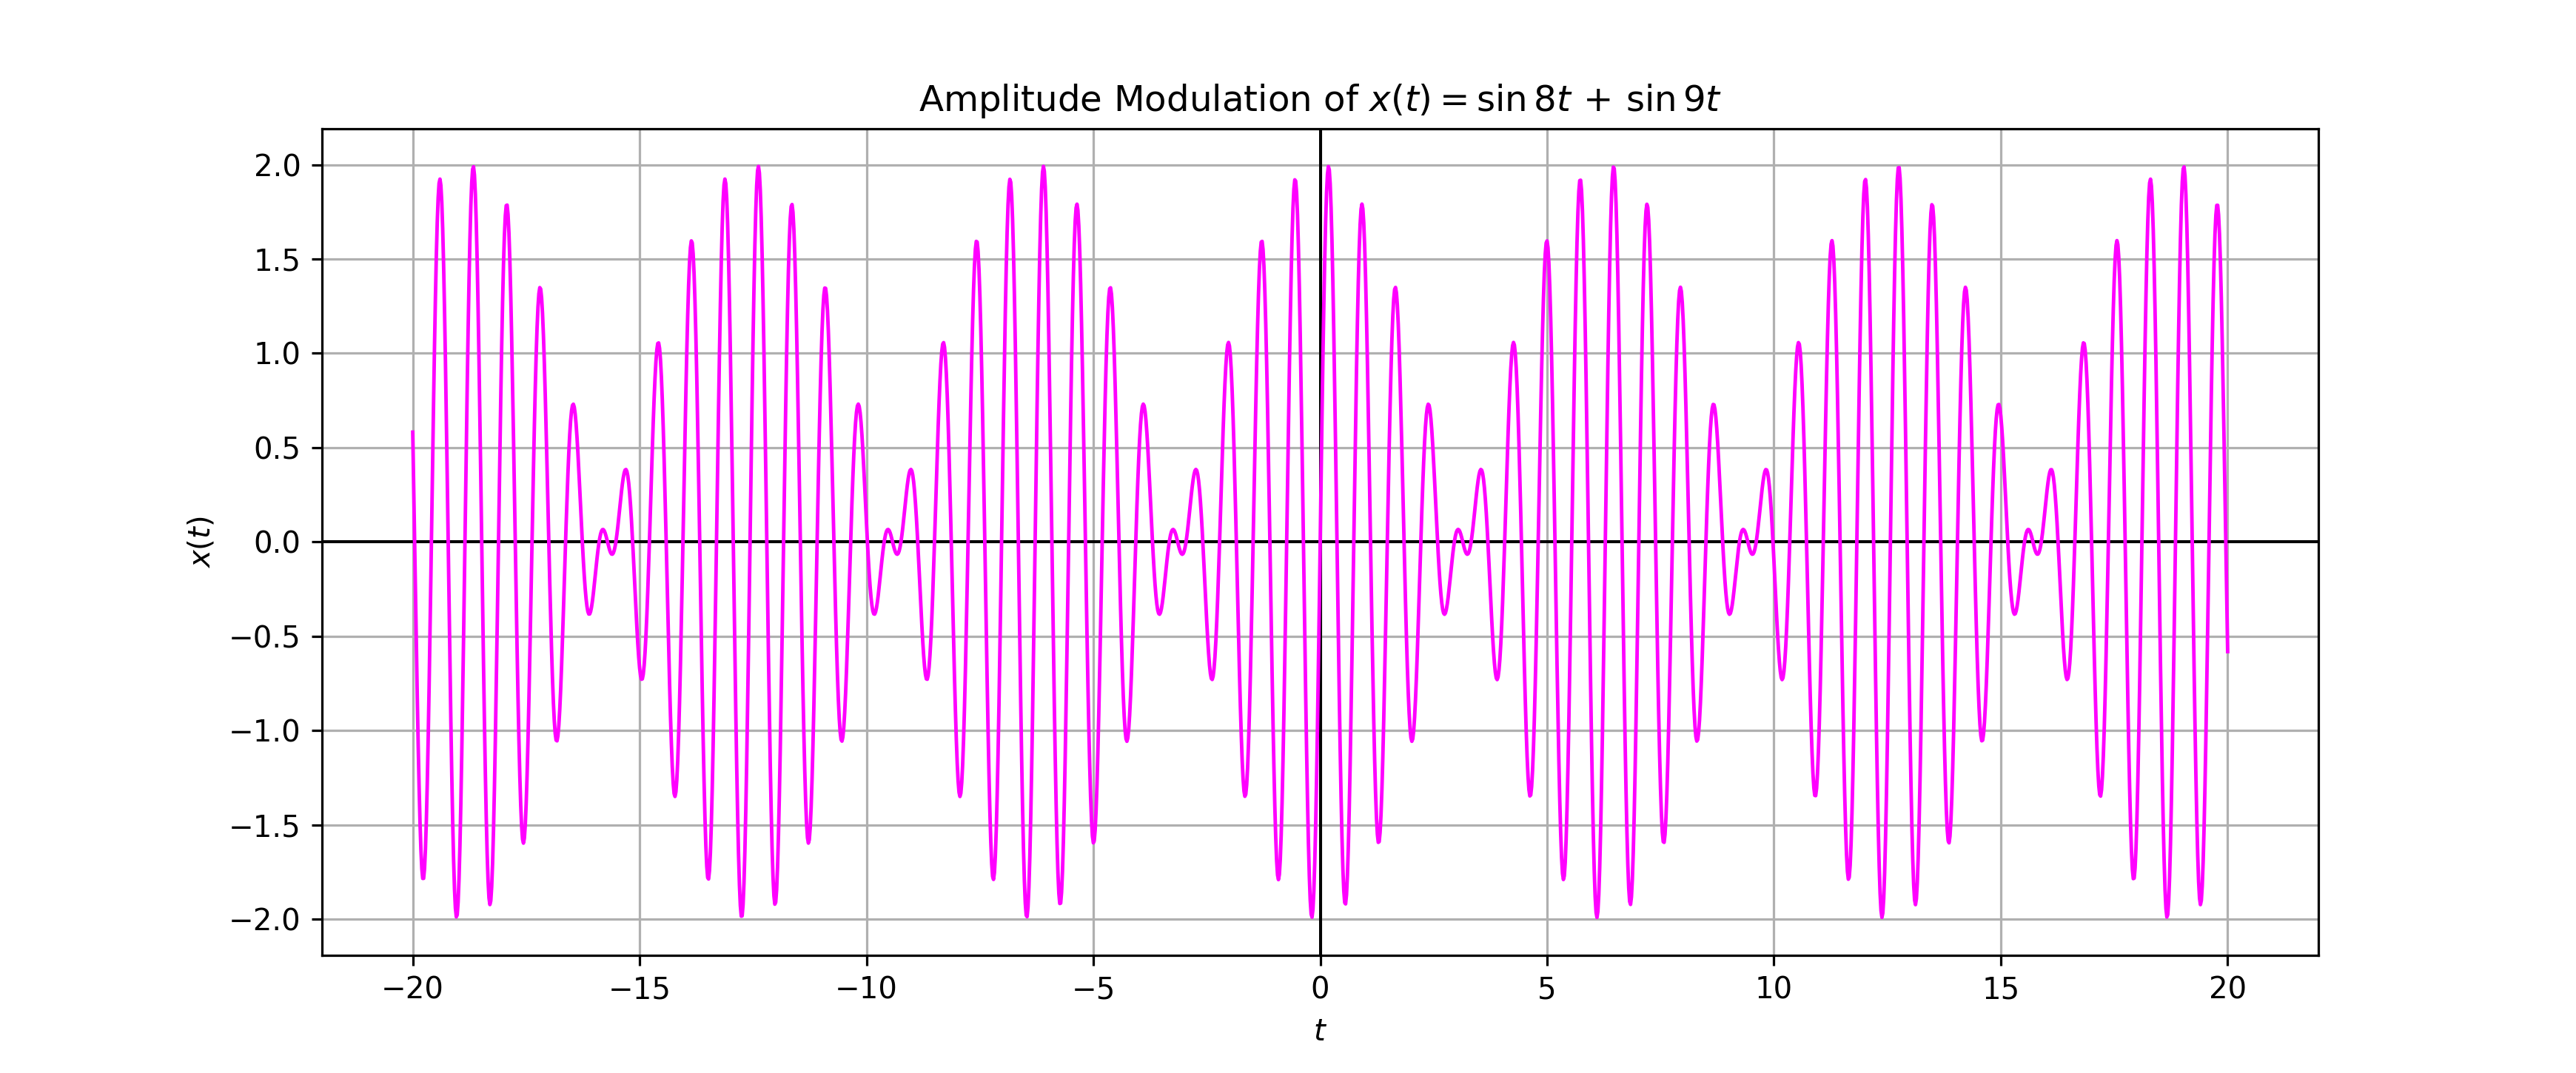
\includegraphics[width=1.1\linewidth]{figs/4.2.2_x.png}
    \caption{\scriptsize{The function $x(t) = \sin{8t} + \sin{9t}$ plotted on the time interval $t\in[-20,20]\,\mathrm{s}$. The amplitude is modulated between $x=0$ and $x=2$. }}
    \label{fig:p4_func}
\end{figure}

\subsection{(a) What is the period of the amplitude modulations? }
\label{ssec:p4a}


By constructive and destructive interference at different times $t$, the amplitude is modulated between $\max{\left|\sin{pt}\right|} + \max{\left|\sin{qt}\right|} = 2$ and $\min{\left|\sin{pt}\right|}+\min{\left|\sin{qt}\right|} = 0$ for an arbitrary constants $p\neq q\in\mathbb{R}$. The period of the constructive and destructive interference is a function of both frequencies of each base wave, which in this case, are $\nu_1 = 8$ and $\nu_2 = 9$. By inspection of Figure \ref{fig:p4_func}, there are roughly $5+2(2/3)\approx 6.33$ periods in an interval of length $40\,\mathrm{s}$, corresponding to a period of about 6.3 s. Since this estimate is very close to $2\pi\approx 6.28$, we estimate a period of $2\pi$. This corresponds to a frequency of $1$, which is equal to the difference of the frequencies $\nu_2-\nu_1$ (as expected).  
\begin{figure}[h]
    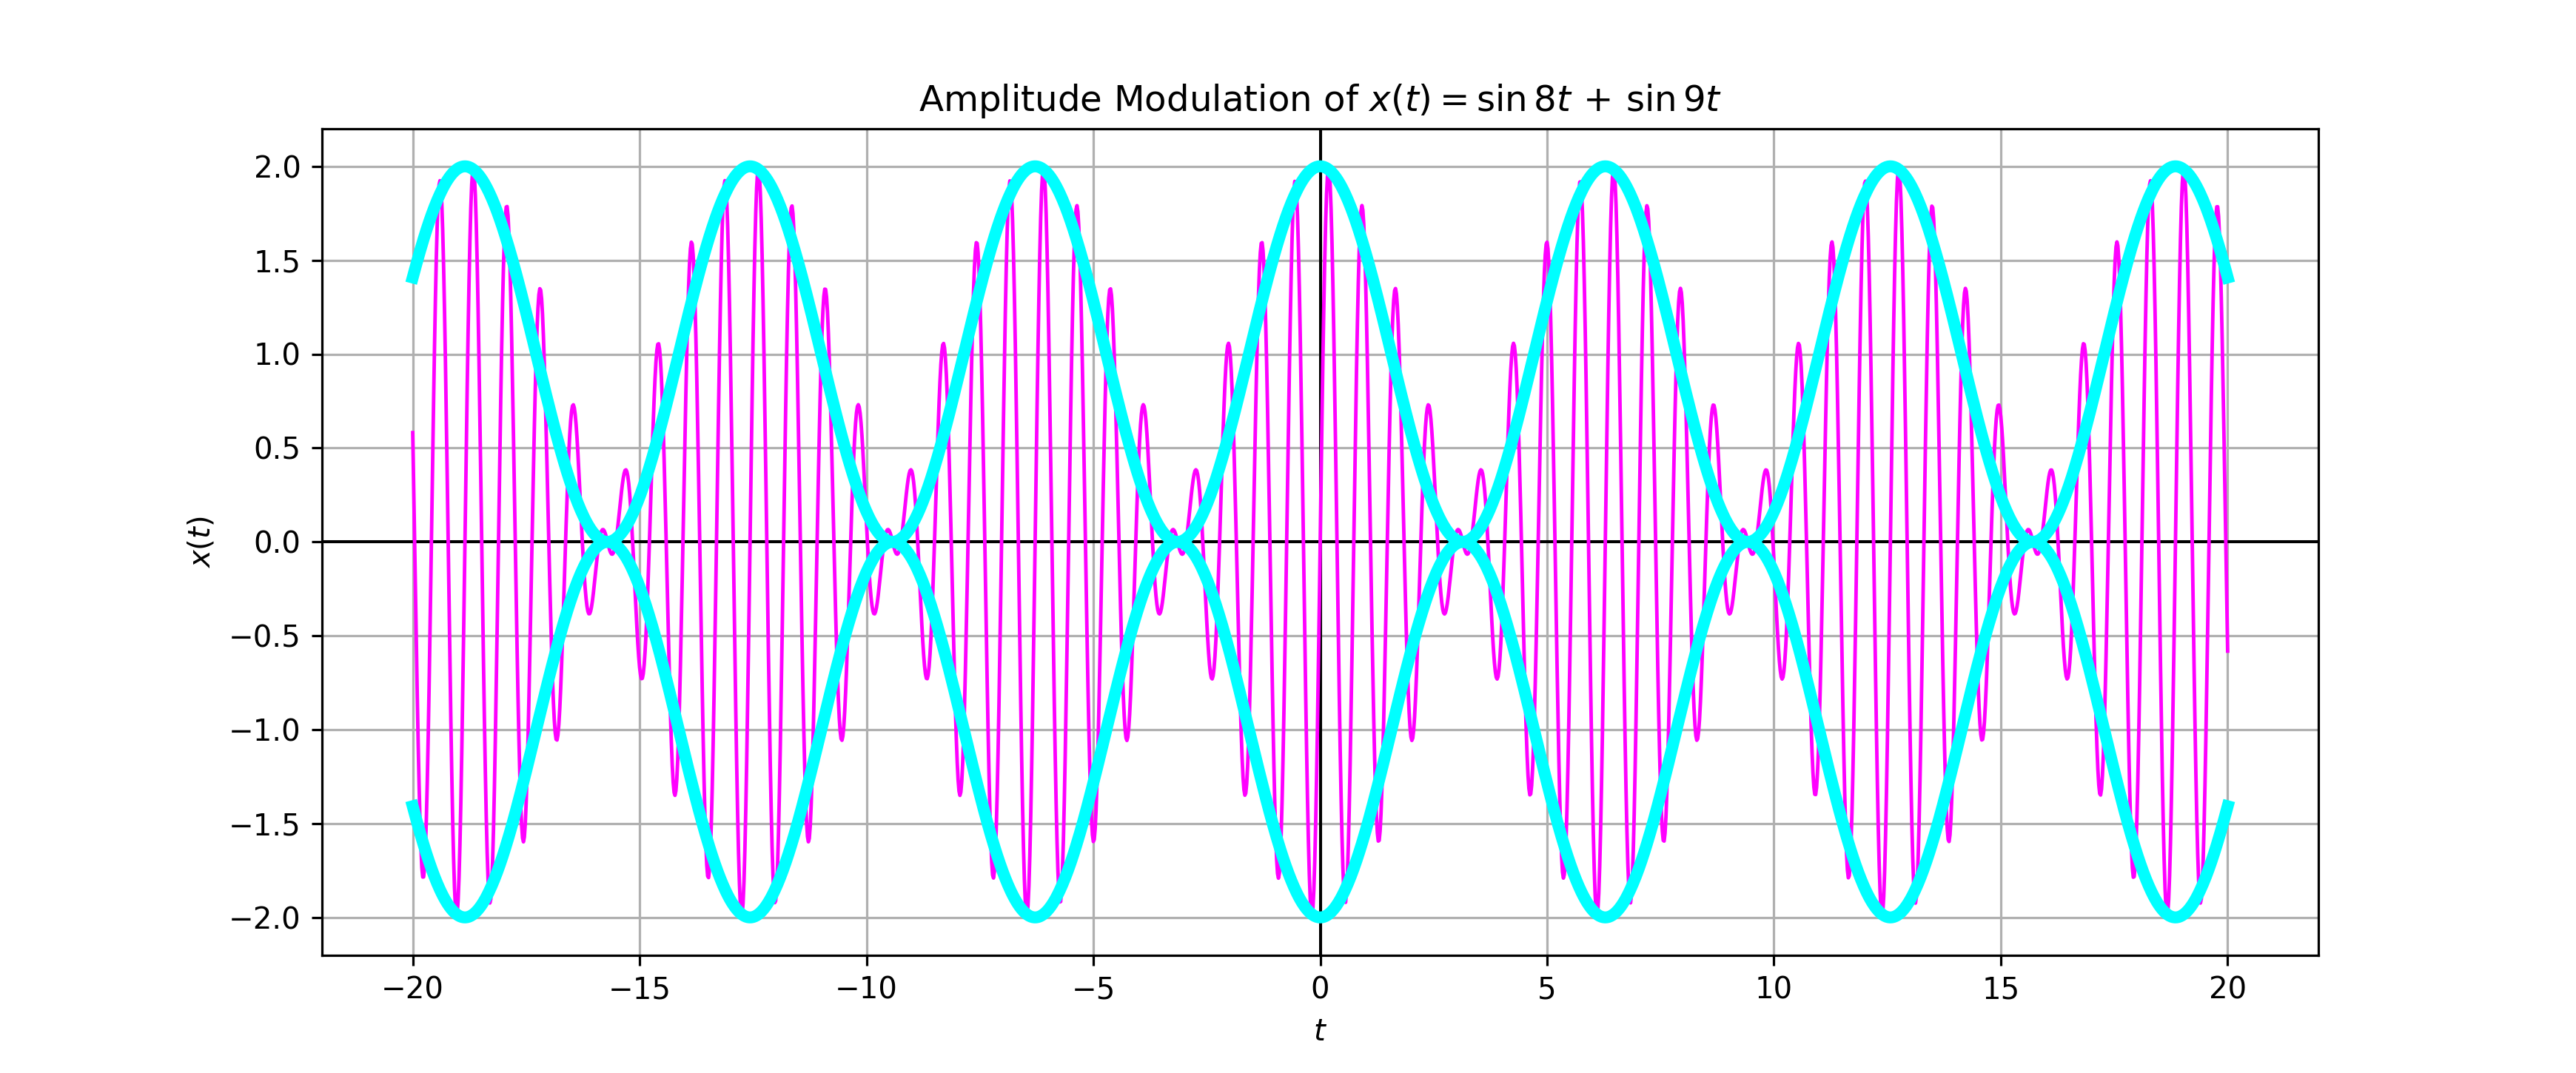
\includegraphics[width=1.1\linewidth]{figs/4.2.2_env.png}
    \caption{\scriptsize{The function $x(t) = \sin{8t} + \sin{9t}$ plotted on the time interval $t\in[-20,20]\,\mathrm{s}$ (magenta), with the envelope of the amplitude modulation $f(t)$ estimated by equation (\ref{eqn:p4_f}) overplotted (cyan). The period of the amplitude modulation is equal to $2\pi$, yielding a frequency of $\nu=1$. }}
    \label{fig:p4_env}
\end{figure}
\par
This can be verified graphically by plotting the \emph{envelope} of the amplitude over the curve in Figure \ref{fig:p4_func}. By inspection of the figure, the ``ansatz" functional form of the envelope is approximately given by 
\begin{equation}
\label{eqn:p4_f}
    f_\pm(t) = \pm (1 + \cos{t}) \qquad , 
\end{equation}
where each ``branch" is restricted to the respective half-space (i.e., $f_+\geq 0$ and $f_-\leq0$).
The expression in equation (\ref{eqn:p4_f}) is shown as the cyan curves of Figure \ref{fig:p4_env}. This envelope assumes that the period of the amplitude modulation corresponds to the time distance between ``peaks".
\par



\subsection{(b) Solve this problem analytically, using a trigonometric identity that converts sums of sines and cosines to products of sines and cosines. }
\label{ssec:p4b}

\begin{figure}[!h]
    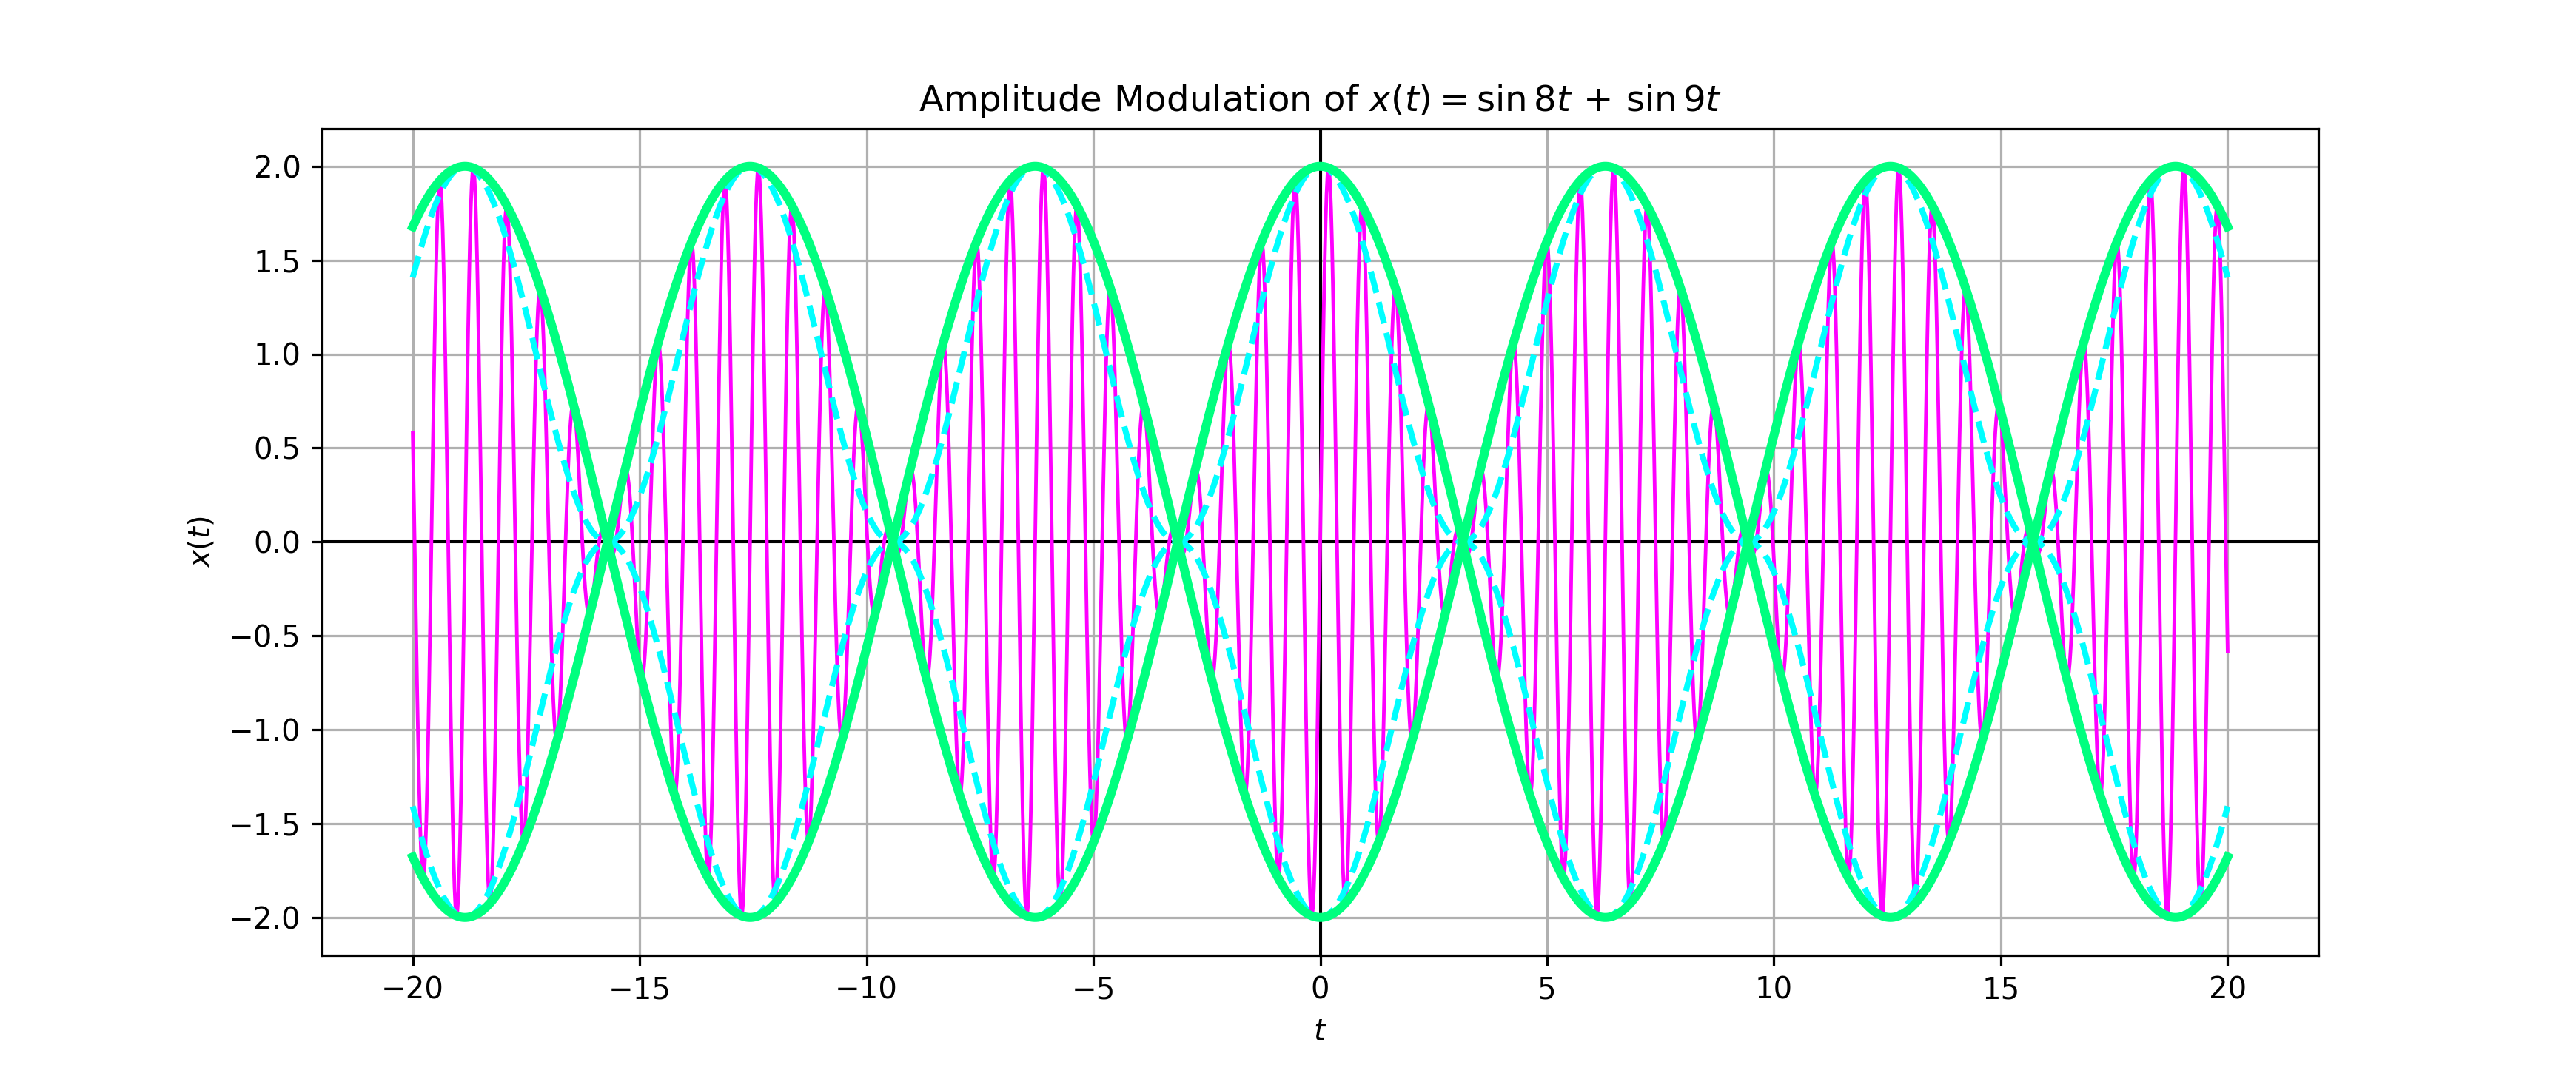
\includegraphics[width=1.1\linewidth]{figs/4.2.2_exact.png}
    \caption{\scriptsize{The function $x(t) = \sin{8t} + \sin{9t}$ plotted on the time interval $t\in[-20,20]\,\mathrm{s}$ (magenta), with the analytically calculated envelope of the amplitude modulation $f(t)$ from equation (\ref{eqn:p4_exact}) overplotted (green). The ansatz for the envelope from section \ref{ssec:p4a} is shown as well (dashed cyan). }}
    \label{fig:p4_exact}
\end{figure}

As recommended, we manipulate
\begin{equation*}
    x(t) = \sin{\nu_1 t} + \sin{\nu_2 t} = \sin{8 t} + \sin{9 t} 
\end{equation*}
using the trigonometric identity 
\begin{equation*}
    \sin{(\theta +\phi)} + \sin{(\theta - \phi)} = 2 \sin{\theta} \cos{\phi} \qquad ,
\end{equation*}
yielding
\begin{equation*}
    x(t) = 2\sin\left(\frac{17t}{2}\right) \cos\left(\frac{t}{2}\right) \qquad .
\end{equation*}
These two factors must correspond to the two simultaneous oscillations occurring between the two terms. By comparison, the one with a higher frequency (i.e., the sine) is not responsible for the oscillation mode of the amplitude modulations. Rather, this must be driven by the cosine factor. Hence, the \emph{exact analytical form} of the envelope we only guessed at in section \ref{ssec:p4a} is given by
\begin{equation}
    \label{eqn:p4_exact}
    f_\pm(t) = \pm \left| 2 \cos\left(\frac{t}{2}\right) \right| \qquad .
\end{equation}
Depending on how the period of the amplitude modulation is defined, whether it corresponds to the period of $\cos{t/2}=4\pi$ or the period of $|\cos{(t/2)}|=2\pi$, the period can be double what we claimed in section \ref{ssec:p4a}. However, we prefer the interpretation that the period refers to the distance between peaks, since these successive peaks and troughs can also be considered as consecutive wavepackets. The curves of equation (\ref{eqn:p4_exact}) are shown in green by Figure \ref{fig:p4_exact}, where the envelope exactly matches the maximums of $x(t)$. The sine term is responsible for the high frequency oscillations that occur within each amplitude-modulated period.
\par









\section{Problem 4.3.6: $\dot \theta = \mu + \sin{\theta} + \cos{2\theta}$.}
\label{sec:p5}

\textbf{Draw the phase portrait as function of the control parameter $\mu$. Classify the bifurcations that occur as $\mu$ varies, and find all the bifurcation values of $\mu$.}

\begin{figure}[!h]
    \centering
    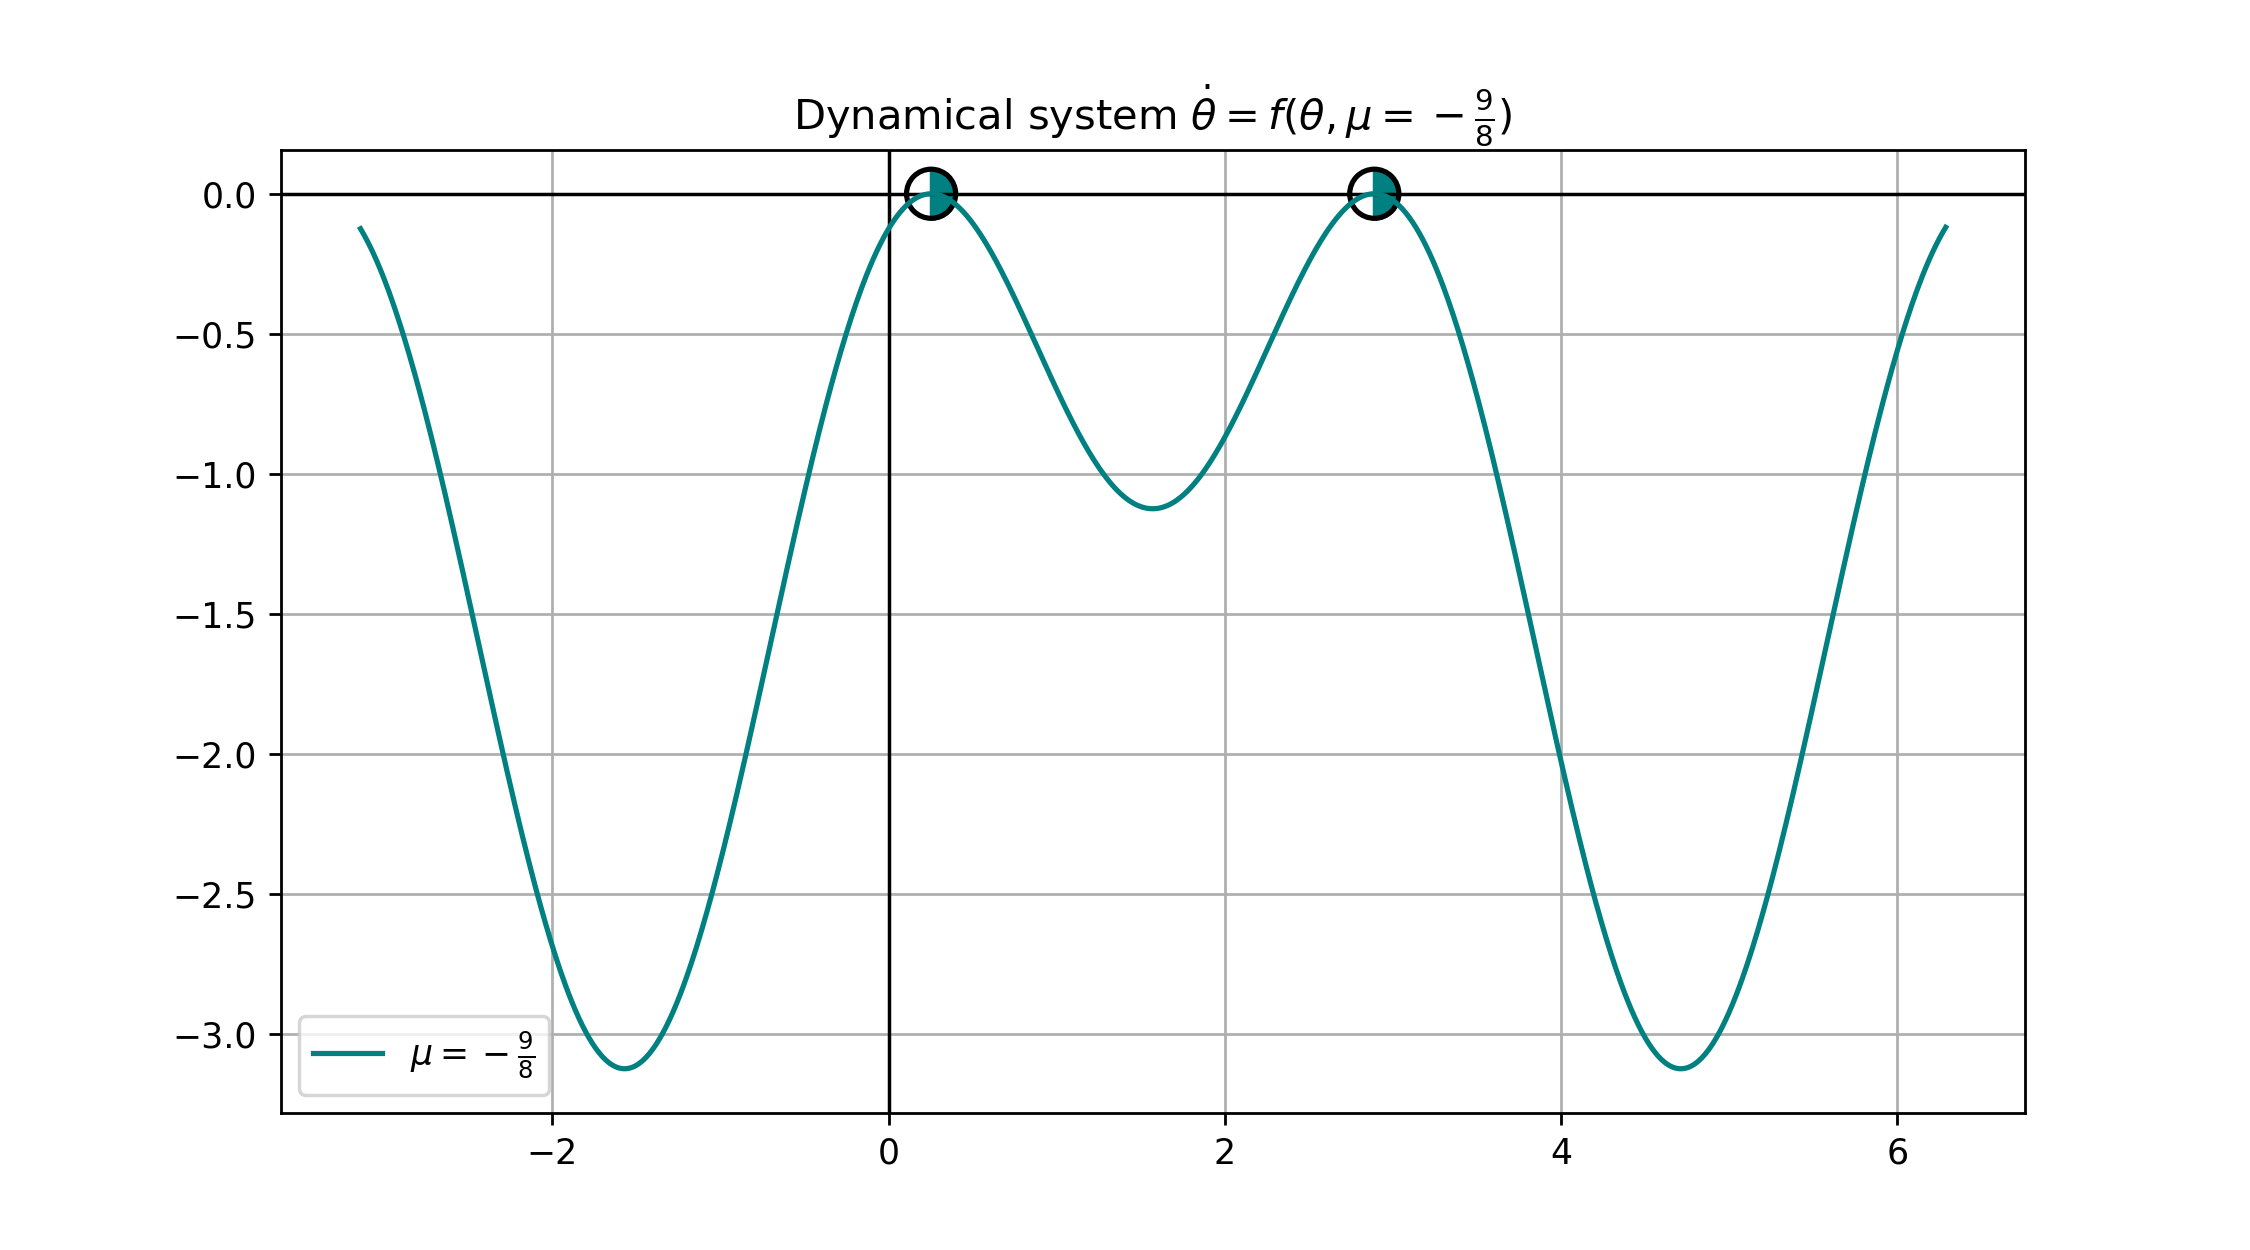
\includegraphics[width=1\linewidth]{figs/4.3.6_muL.png}
    \caption{\scriptsize{Dynamical system given by $f(\theta,\mu) = \mu + \sin{\theta} + \cos{2\theta}$ for $\mu=-9/8$. This phase portrait shows the instant that a bifurcation unfolds.  }}
    \label{fig:p5_muN}
\end{figure}



To investigate this system, we define $g(\theta)$:
\begin{equation*}
    f(\theta,\mu) = \mu + \sin{\theta} + \cos{2\theta} \equiv \mu + g(\theta) \qquad .
\end{equation*}
To determine the range of $\mu$ for which there are fixed points $\dot \theta = 0$, we must calculate the locations and values of the extrema of $g(\theta)$. To do so, we start with
\begin{equation*}
    \max g(\theta) \longrightarrow g(\theta_m) \quad : \quad g'(\theta_m) = 0 \quad , \quad g''(\theta_m)<0 \quad .
\end{equation*}
Then, differentiating $g$
\begin{equation*}
    g'(\theta) = \cos{\theta} - 2 \sin{2\theta} \quad , 
\end{equation*}
which implies that 
\begin{equation*}
    0 = \cos{\theta_m} - 2 \sin{2\theta_m} \quad \implies \quad \tan{2\theta_m} = \frac{1}{2} \qquad .
\end{equation*}
Thus, we have that the extrema are located at 
\begin{equation*}
    \theta_m = \frac{1}{2} \arctan{\left(\frac{1}{2}\right)} \qquad .
\end{equation*}
Substituting this into $g(\theta)$, we find 
\begin{equation*}
    \max{g(\theta)} = g(\theta_m) = \sin{\left(\frac{1}{2} \arctan{\left(\frac{1}{2}\right)}\right)} + \cos{\left(\arctan{\left(\frac{1}{2}\right)}\right)} = \frac{9}{8} \qquad .
\end{equation*}
By the symmetry of the function $g$, another maximum exists at $\theta=\pi-\theta_m$.
\par
\begin{figure}
    \centering
    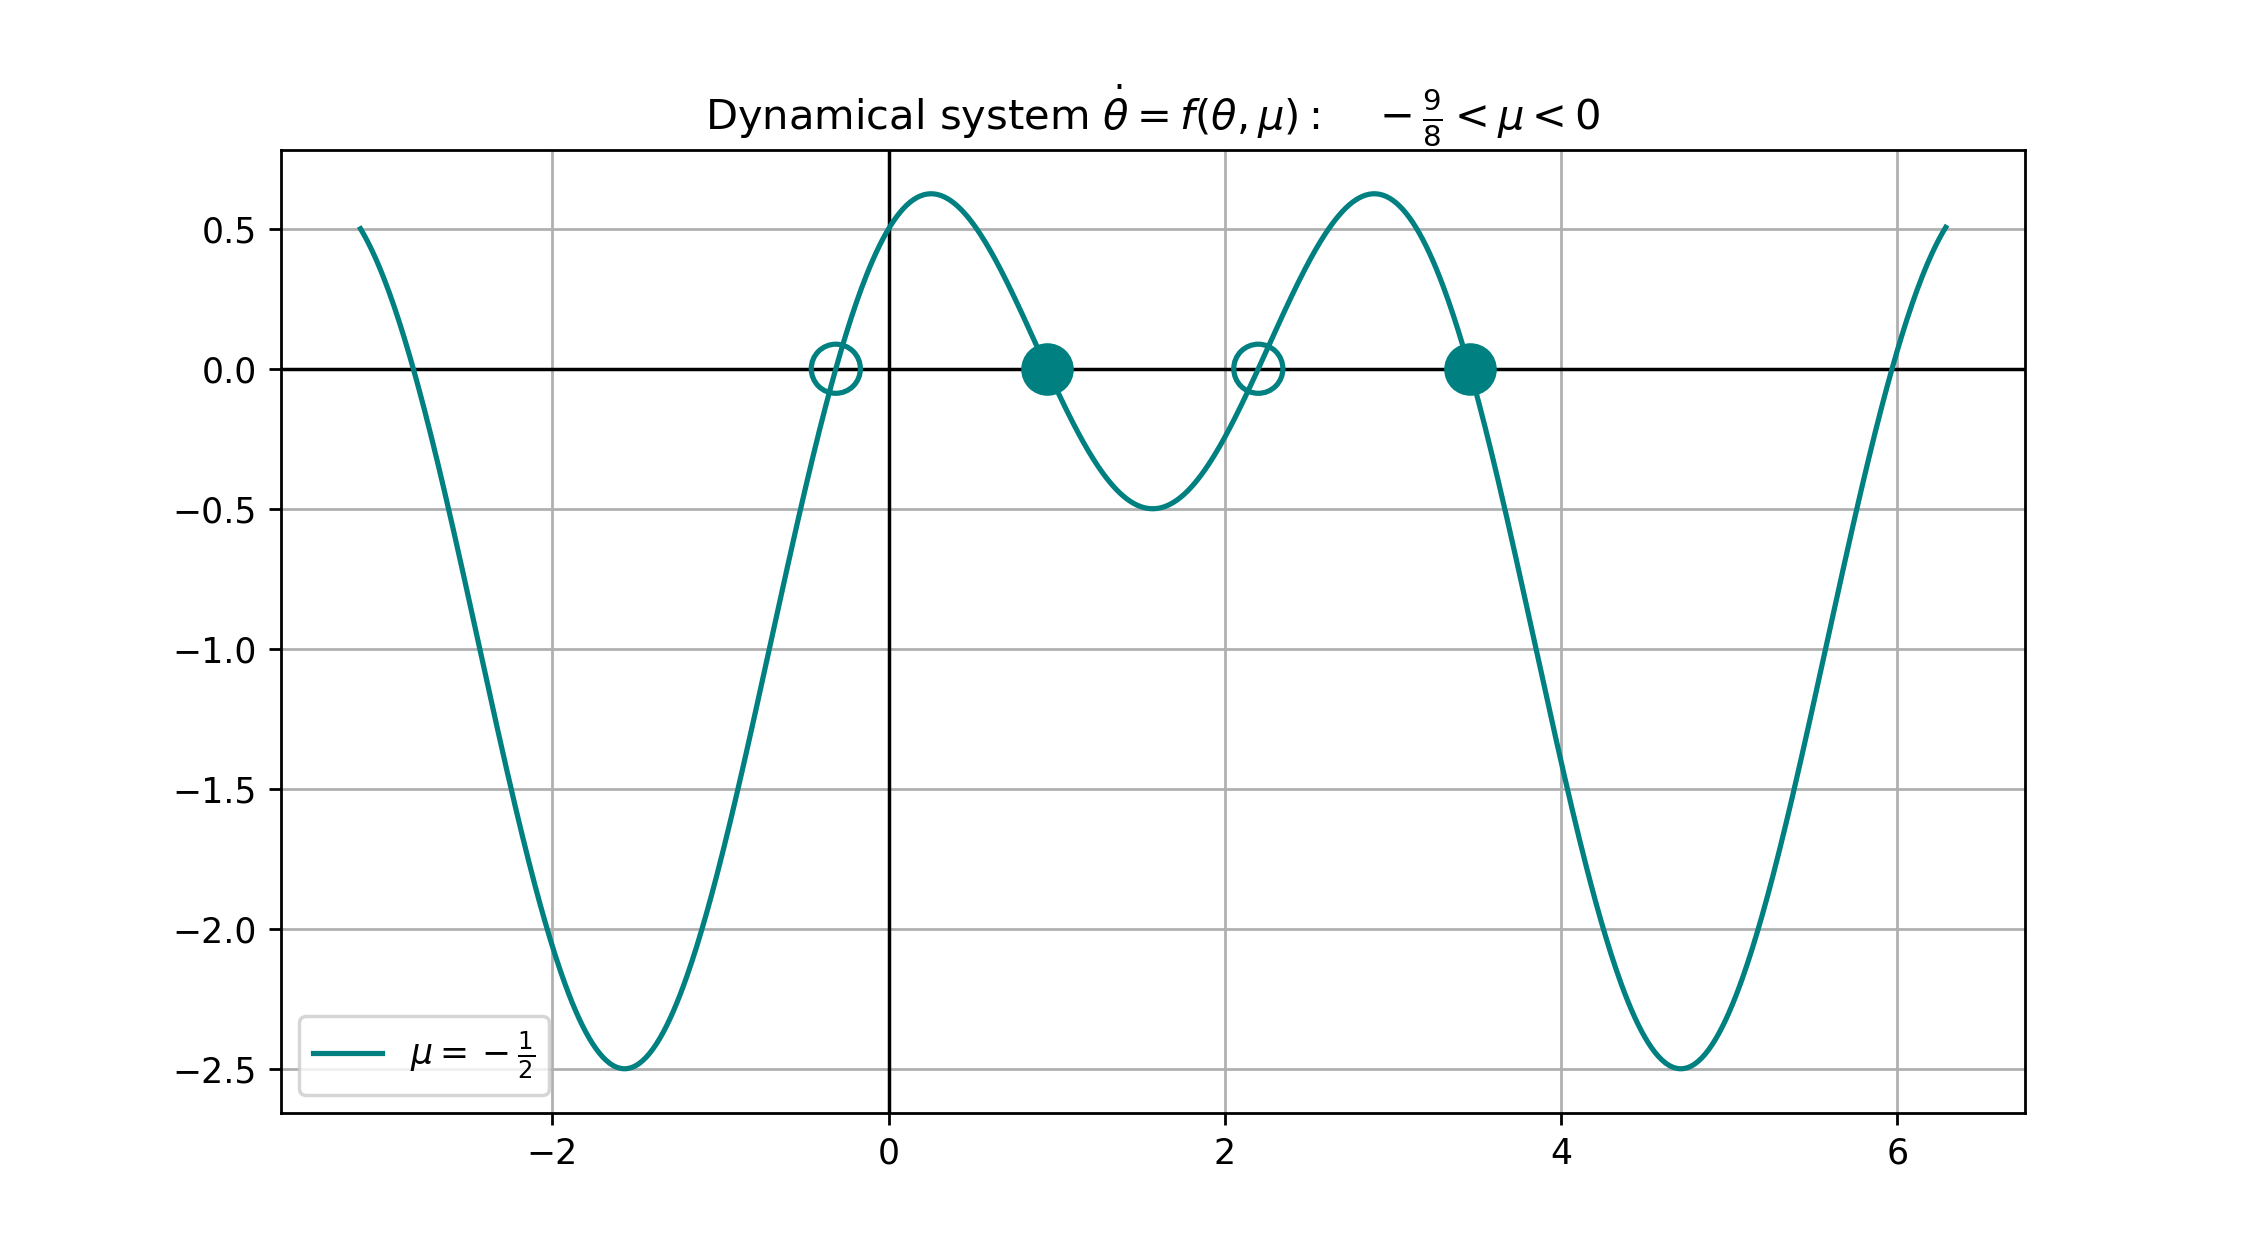
\includegraphics[width=1\linewidth]{figs/4.3.6_muLm.png}
    \caption{\scriptsize{Dynamical system given by $f(\theta,\mu) = \mu + \sin{\theta} + \cos{2\theta}$ for $\mu=-1/2$. This phase portrait shows the moments after the bifurcation from Figure \ref{fig:p5_muN}.  }}
    \label{fig:p5_muL0}
\end{figure}


On the other hand, the minimum is given in the ``third" quadrant of the unit circle, since this is where both $\sin{\theta}$ and $\cos{\theta}$ are negative. At $\theta_l=3\pi/2$, $g(\theta_l)=-2$. Because sine and cosine can only have an absolute value of at most unity, this represents the minimum value of $g$. In contrast, at $g(\pi/2)$ the double frequency cosine term actually \emph{negates} the sine term, creating a local minimum with $g(\theta=\pi/2)=0$.
Thus, given the range that $g$ spans, we have determined that for $\mu>2$ or $\mu < (-9/8)$, there exist no roots of $\dot \theta=f(\theta,\mu)$. In these cases, $|\mu| > |g(\theta)|$. We consider the phase portraits as a function of $\mu$, and use them to classify each bifurcation. We consider $\mu$ \emph{increasing} as the ``forward" direction in this analysis.
\par
\begin{figure}
    \centering
    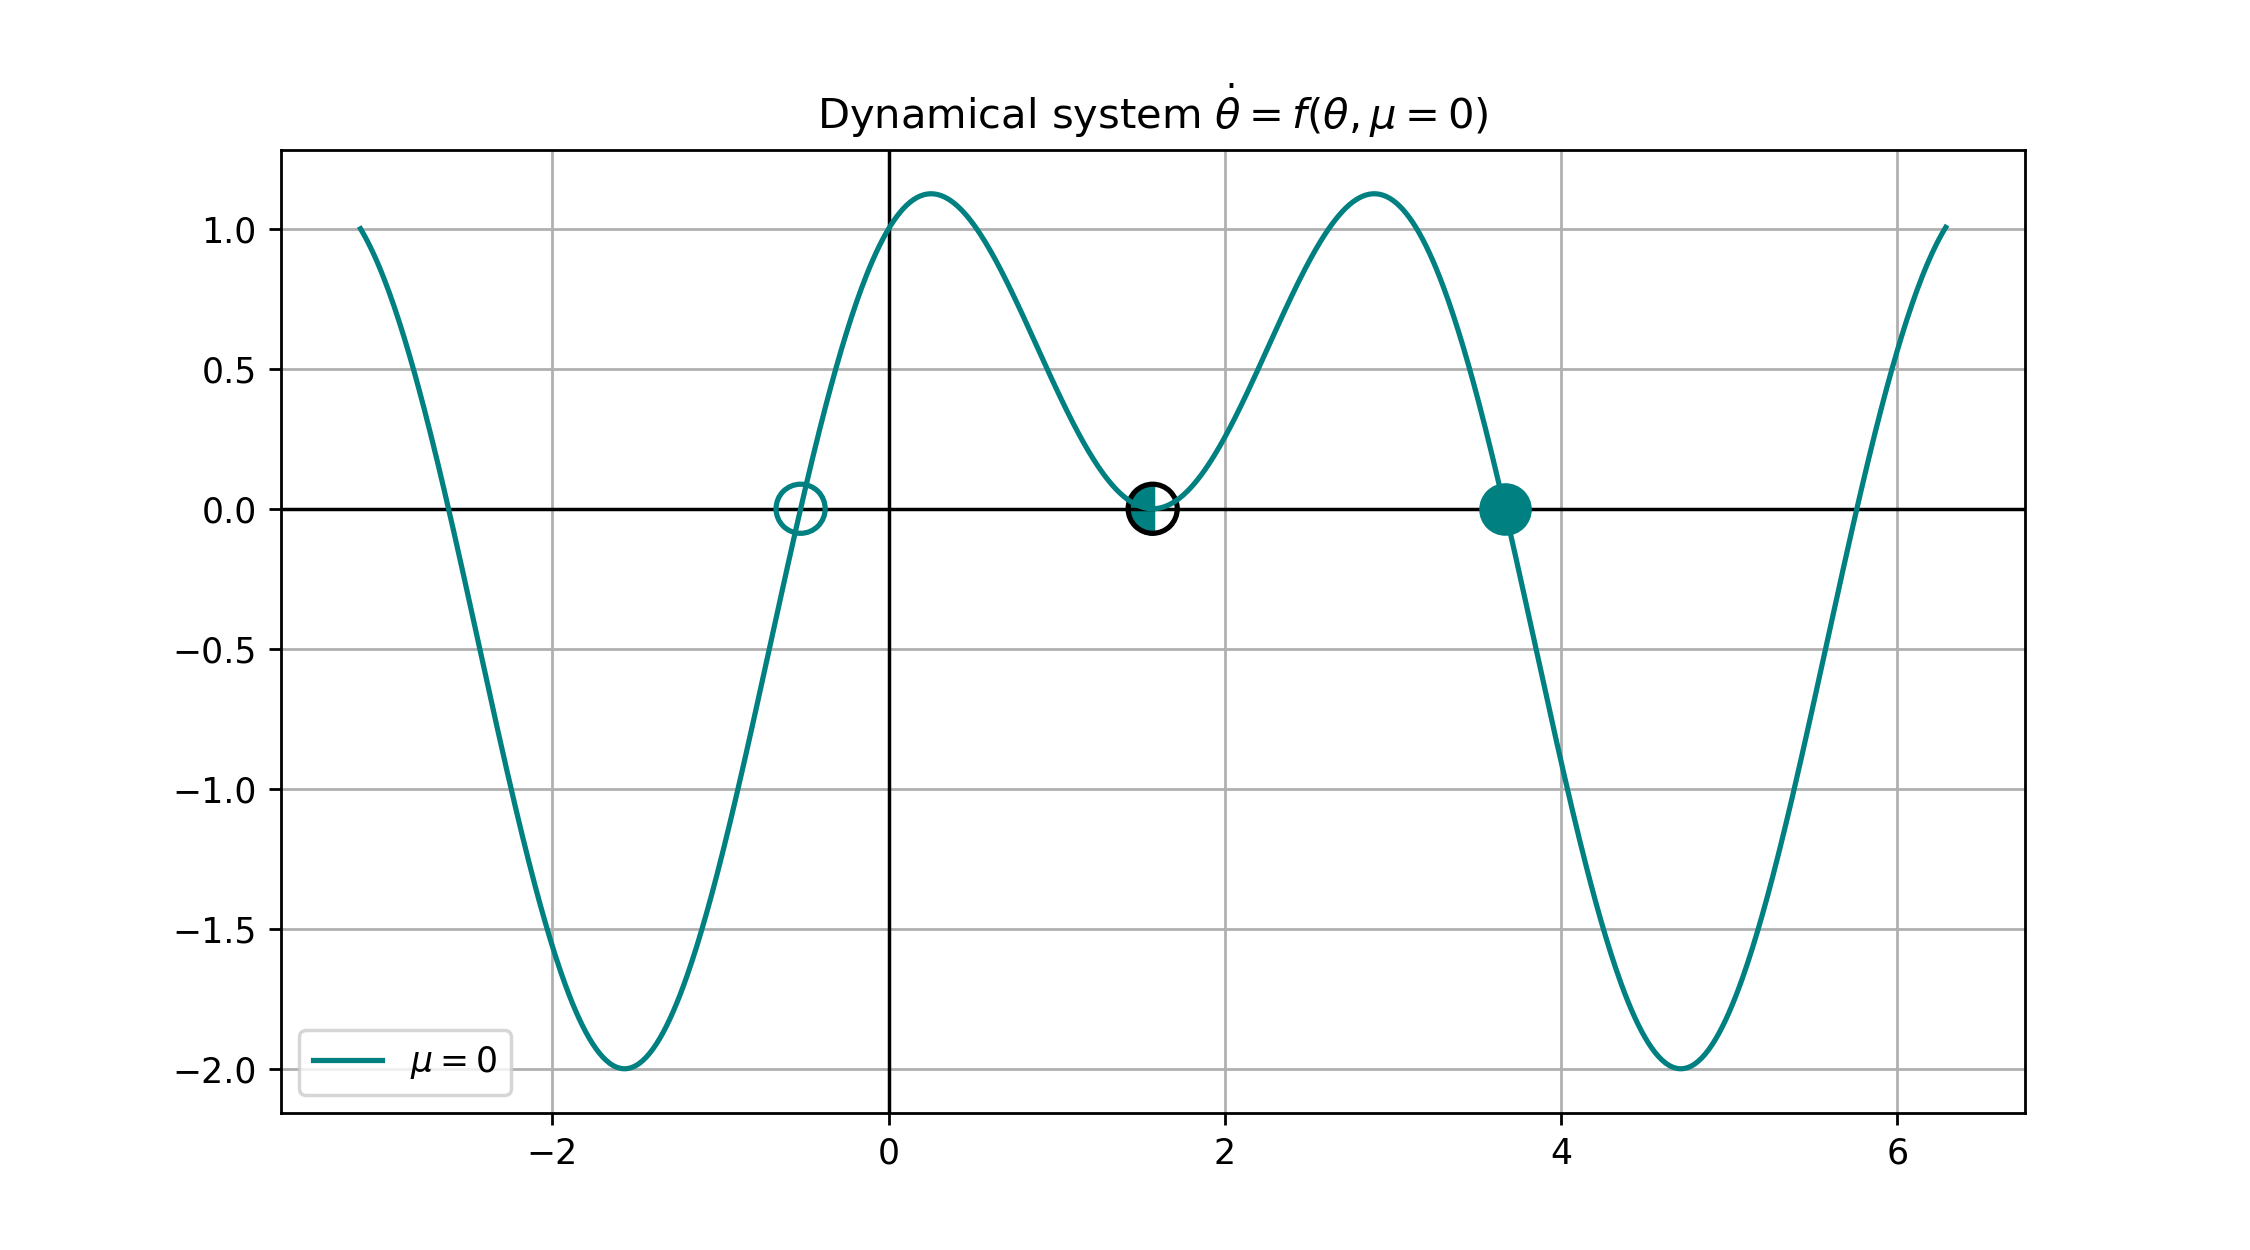
\includegraphics[width=1\linewidth]{figs/4.3.6_muE0.png}
    \caption{\scriptsize{Dynamical system of $f(\theta,\mu) = \mu + \sin{\theta} + \cos{2\theta}$ for the parameter $\mu=0$. This phase portrait shows the moment a \emph{second} bifurcation occurs.  }}
    \label{fig:p5_muE0}
\end{figure}


Hence, to determine the bifurcations of this system, we compute the phase portrait of $f$ as a function of $\mu\in[\,-9/8\,,2]$. To start, we consider the first bifurcation when $\mu$ passes through $\mu=-9/8$. As $\mu$ increases, 2 semi-stable fixed points are created, as evidenced by Figure \ref{fig:p5_muN}. Each semi-stable fixed point corresponds to the minimum of $g(\theta)$, and two fixed points are created from each one of the semi-stable fixed point with increasing $\mu$. This process of the single fixed point producing a pair of fixed points, one stable and one unstable, is common for a saddle node bifurcation. This instance actually is consistent with the definition of a blue-sky bifurcation.
\par
\begin{figure}
    \centering
    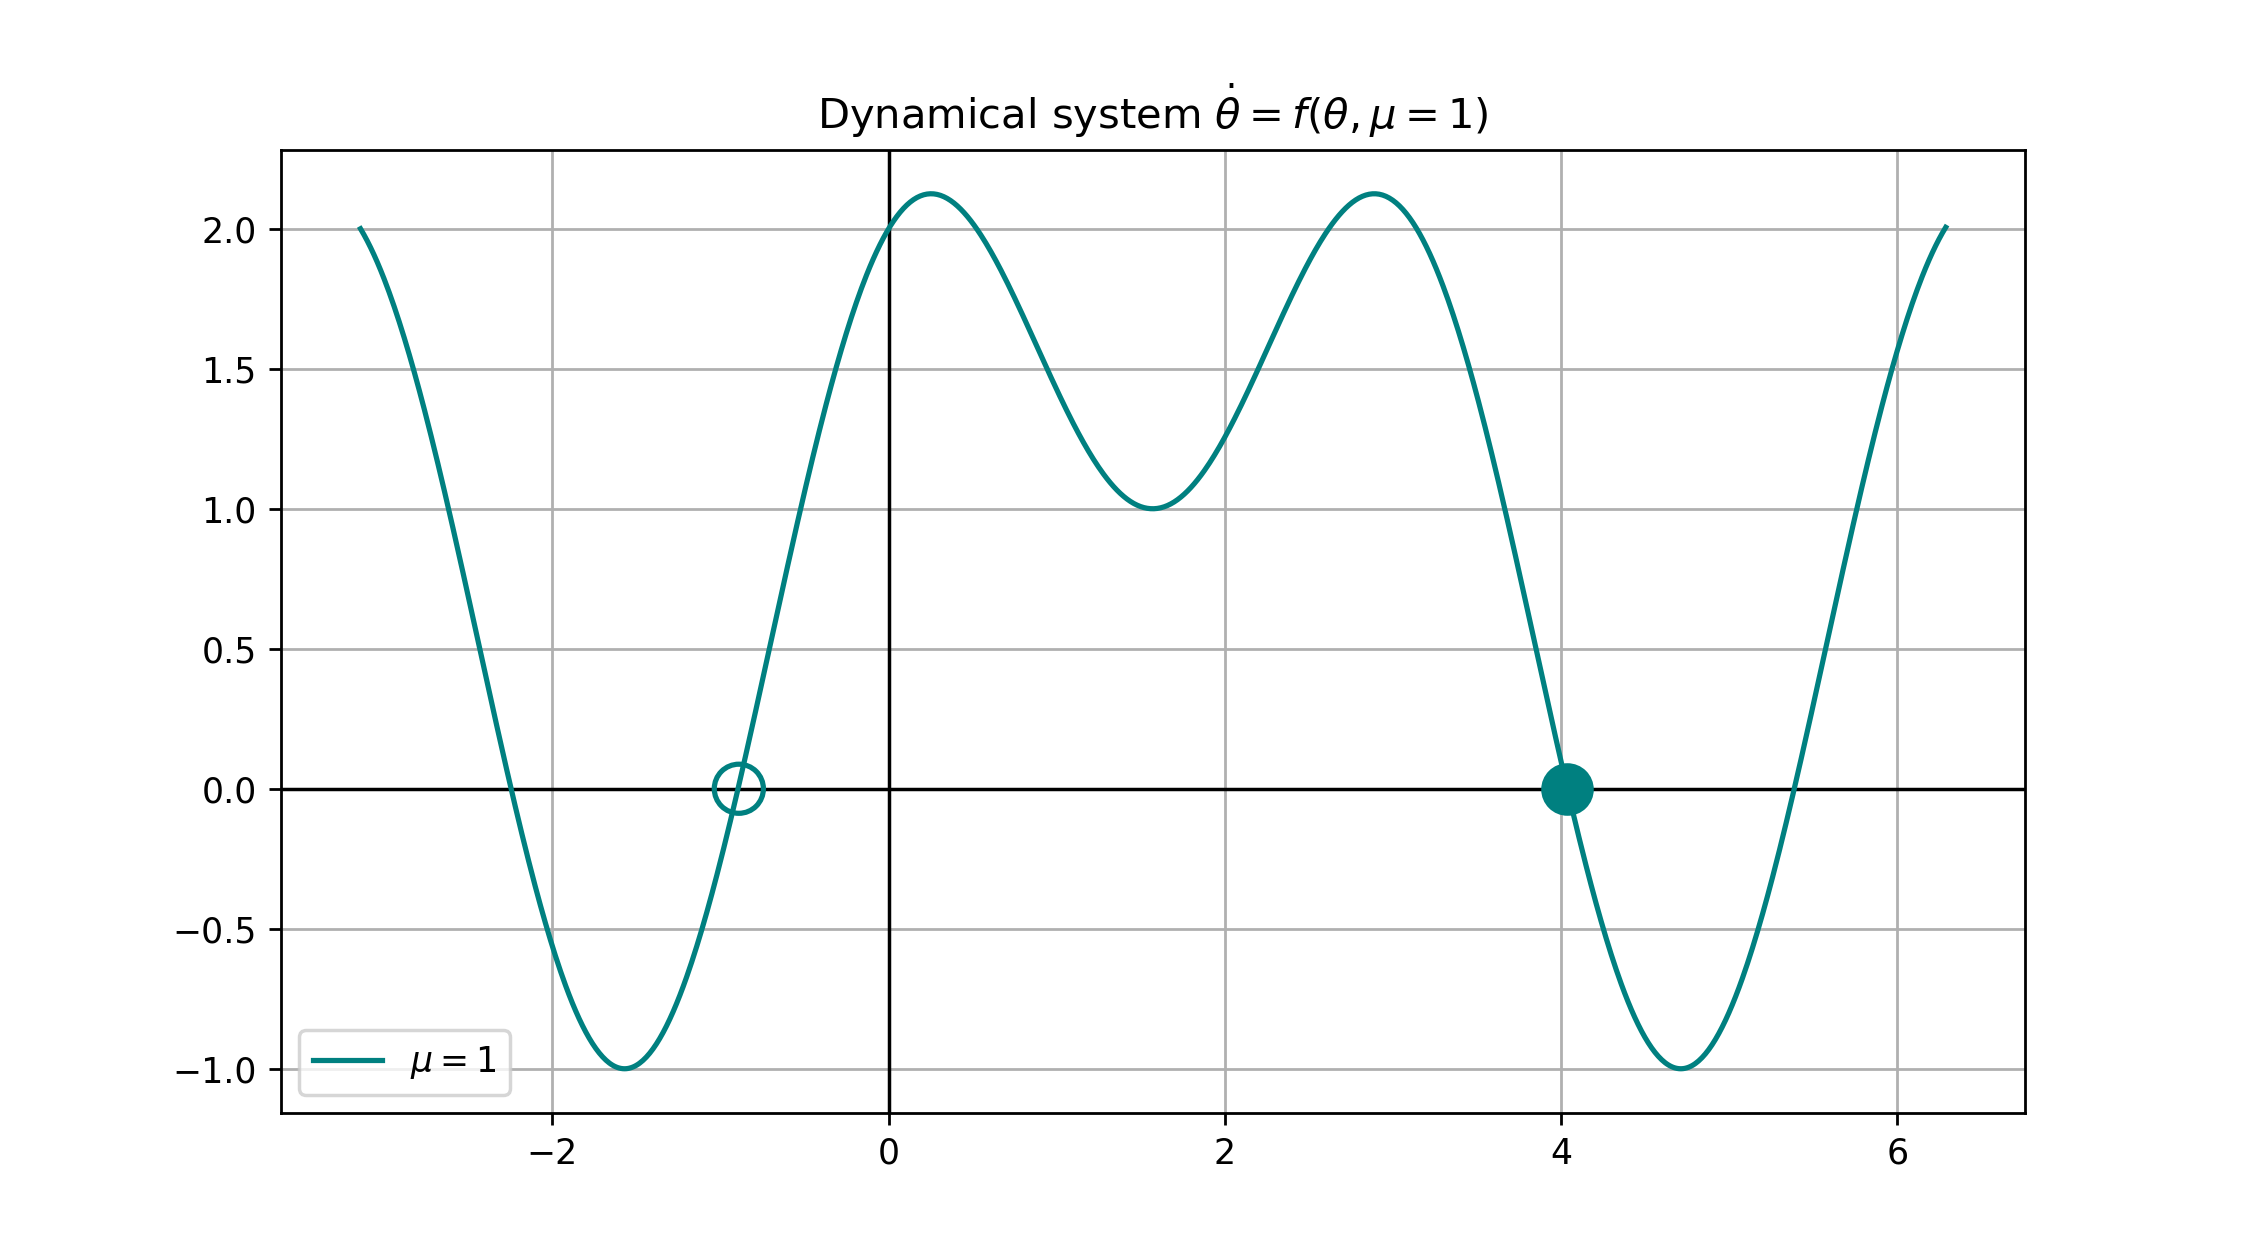
\includegraphics[width=1\linewidth]{figs/4.3.6_mu1.png}
    \caption{\scriptsize{Dynamical system of $f(\theta,\mu) = \mu + \sin{\theta} + \cos{2\theta}$ for the parameter $\mu=1$. This phase portrait shows the fixed points created from the \emph{second} blue-sky bifurcation (see Figure \ref{fig:p5_muE0}.  }}
    \label{fig:p5_muG0}
\end{figure}

Next, we consider what happens when the second, local minimum of $g(\theta)$ encounters the $\dot \theta = 0$ axis. This occurs when $\mu = 0$. Hence, we show in Figure \ref{fig:p5_muE0} the system for $f(\theta,0)=g(\theta) = \dot \theta$. At this point, it is evident that a \emph{second} bifurcation occurs, as another semi-stable fixed point originates in addition to the previously created pair. This second blue-sky bifurcation creates another pair of stable and unstable fixed points. 
\par
However, as shown by the marker in Figure \ref{fig:p5_muE0}, the stable direction (the side that the stable fixed point will be created on) is from lower values of $\theta$, in contrast to the ones produced in Figure \ref{fig:p5_muN}. This is further illustrated in Figure \ref{fig:p5_muG0}, where the aftermath of the second blue-sky bifurcation is depicted for a value of $\mu=1$.
\par
\begin{figure}
    \centering
    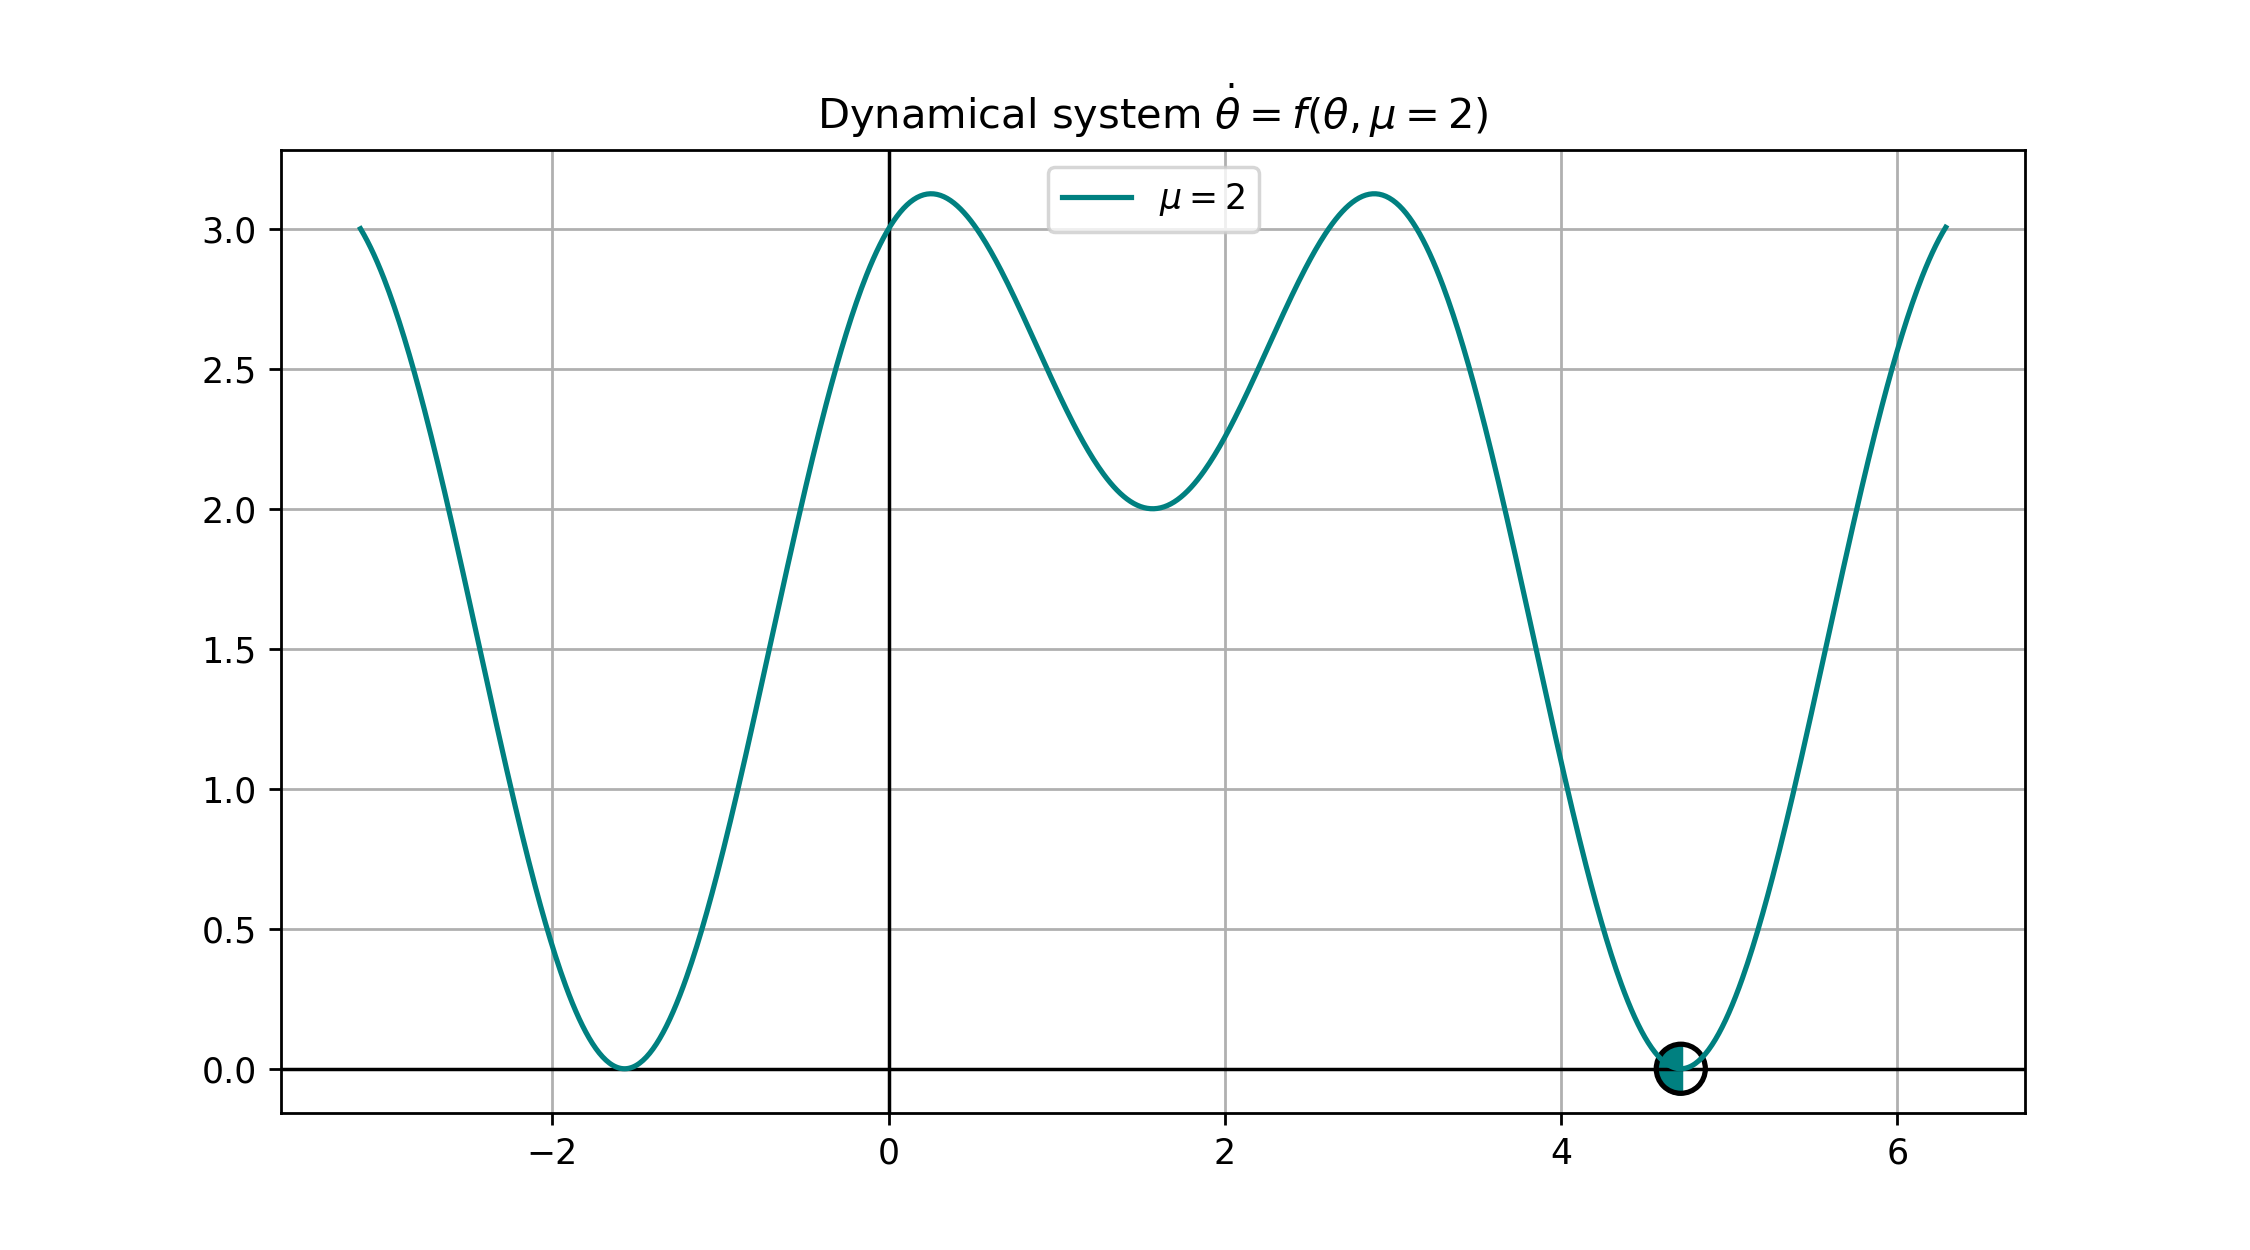
\includegraphics[width=1\linewidth]{figs/4.3.6_mu2.png}
    \caption{\scriptsize{Dynamical system governed by $f(\theta,\mu) = \mu + \sin{\theta} + \cos{2\theta}$ for the parameter value $\mu=2$. .  }}
    \label{fig:p5_muE2}
\end{figure}

Finally, we consider the other extreme, when $\mu=2$. This case is shown in Figure \ref{fig:p5_muE2}, where only a single, semi-stable fixed point remains. Hence, two saddle-node (or blue sky) bifurcations occur as $\mu$ varies from $\mu<-9/8$ to $\mu>2$.













\section{Problem 4.4.1: Validity of the Overdamped Limit}
\label{sec:p6}

\textbf{Find the conditions under which it is valid to approximate the equation $mL^2 \ddot \theta + b \dot \theta + MgL \sin{\theta}=\Gamma$ by its overdamped limit $ b \dot \theta + MgL \sin{\theta}=\Gamma$.}

To do so, we consider the scaling of each factor including the time derivatives on $\theta$. To this end, let $t\longrightarrow \tau/c$ for some constant $c$ to be specified at a later point. Then, the governing equation becomes, with the substitution $\mathrm{d}t = \frac{1}{c}\mathrm{d}\tau$, 
\begin{equation*}
    \implies m L^2 c^2 \frac{\mathrm{d}^2\theta}{\mathrm{d}\tau^2} + b c \frac{\mathrm{d}\theta}{\mathrm{d}\tau} + m g L \sin{\theta} = \Gamma \qquad .
\end{equation*}
After a bit of manipulation (and switching back to Newton's notation for the time derivatives), we have
\begin{equation*}
    \frac{L c^2}{g} \ddot \theta + \frac{b c}{m g L} \dot \theta + \sin{\theta} = \frac{\Gamma}{m g L} \qquad ,
\end{equation*}
which gives us the ability to compare each term to $\sin{\theta}$, on the order of unity. If we let $c\equiv mg L/b$, then we find
\begin{equation*}
    \frac{Lc^2}{g} \ddot \theta + \dot \theta + \sin{\theta} = \frac{\Gamma}{m g L} \qquad .
\end{equation*}
Hence, we must have a condition on the leading factor of the $\ddot \theta$ term, keeping it well below the order of unity (the other two terms on the LHS). If the factor 
\begin{equation*}
    \frac{Lc^2}{g} = \frac{L^3 m^2 g}{b^2} \ll 1 \qquad ,
\end{equation*}
then we can safely neglect the $\ddot \theta$ term for arbitrary $\theta$. This allows the governing equation of the (dampened and forced) harmonic oscillator (see prompt) to be rewritten as
\begin{equation*}
    b \dot \theta + MgL \sin{\theta}=\Gamma \qquad ,
\end{equation*}
that is, in its overdamped limit. Hence, possibly as expected, dampening depends not only on the viscous coefficient $b$ but also the length scale $L$ as well as $m$ and $g$. 




\section{Problem 4.5.1: Triangle Wave}
\label{sec:p7}

In the firefly model, the sinusoidal form of the firefly’s response function was chosen somewhat arbitrarily. Consider the alternative model
\begin{equation*}
    \dot \Theta = \Omega , \quad  \dot \theta = \omega + A f(\Theta -\theta)
\end{equation*}
where $f$ is now given by a triangle wave. Let 
\begin{equation}
\label{eqn:p7}
\begin{array}{cc}
  f(\phi)= \Bigg\{ & 
    \begin{array}{cc}
      \phi\,,\, \qquad -\frac{\pi}{2} \leq \phi \leq \frac{\pi}{2}\\
      \pi - \phi \,,\, \qquad \frac{\pi}{2} \leq \phi \leq \frac{3\pi}{2} \\
    \end{array}
\end{array}
\end{equation}
where $f$ is extended periodically beyond this interval. 


\subsection{(a) Graph $f(\phi)$. }
\label{ssec:p7a}

The response function $f$ from equation (\ref{eqn:p7}) is plotted on the specified interval in Figure \ref{fig:p7}. The period of the triangle wave visible in Figure \ref{fig:p7} can be extended infinitely many times to produce a periodic function defined on an arbitrary interval of $\phi$. 
\par
\begin{figure}[!h]
    \centering
    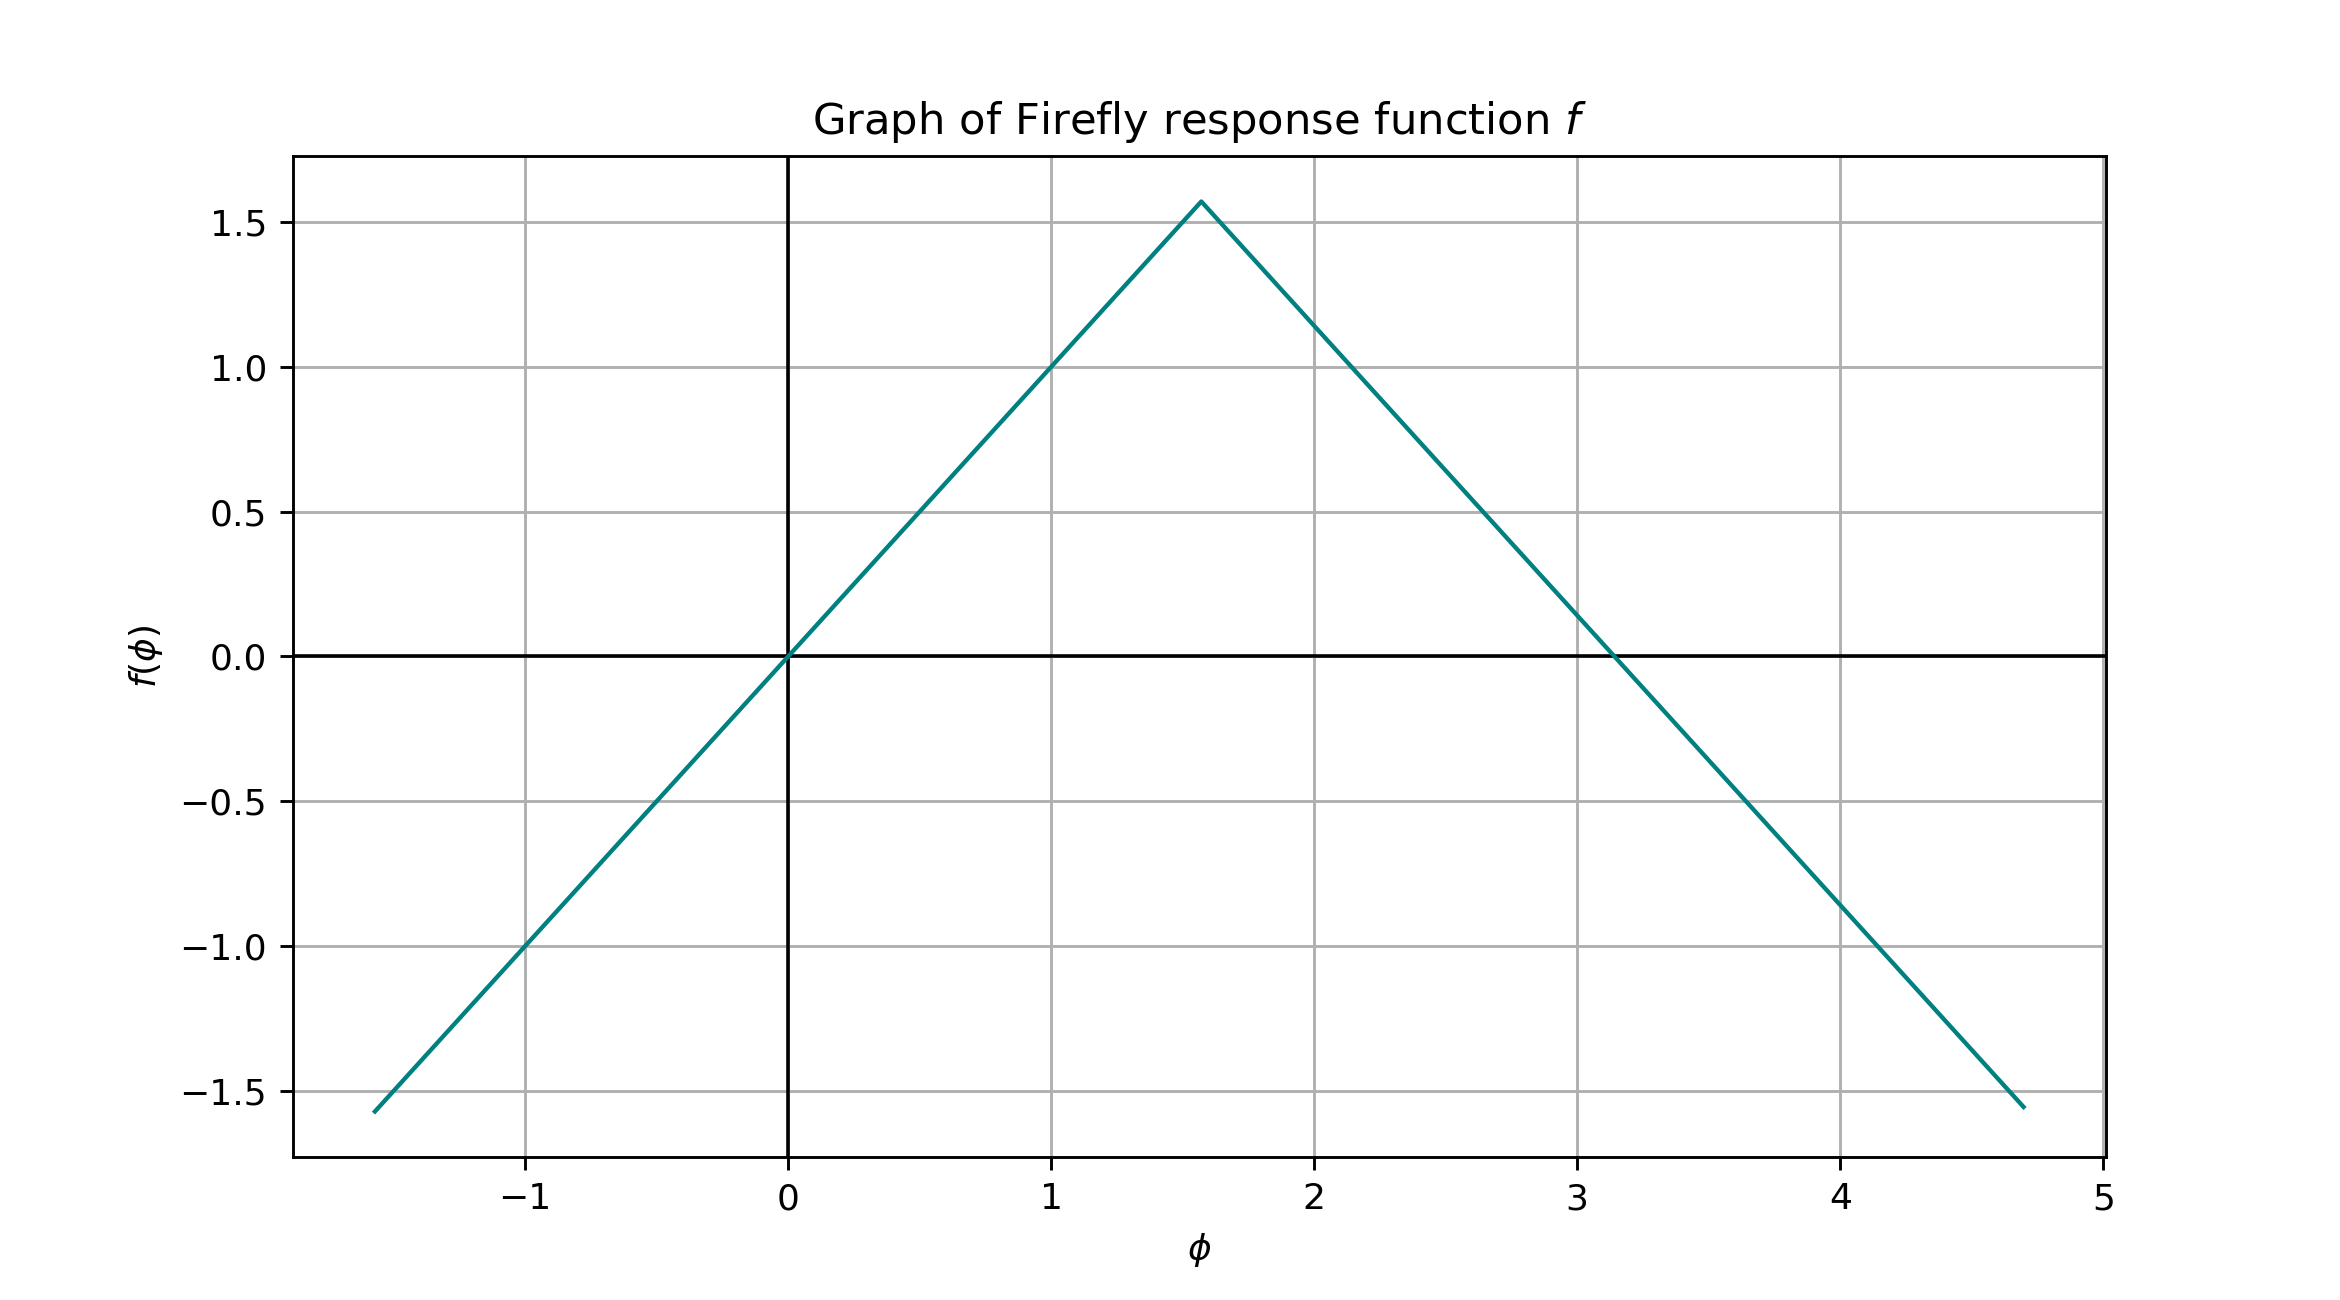
\includegraphics[width=0.75\linewidth]{figs/p7_f.png}
    \caption{Firefly response function $f(\phi)$ given by equation (\ref{eqn:p7}).}
    \label{fig:p7}
\end{figure}



\subsection{(b) Find the range of entrainment. }
\label{ssec:p7b}

Following the approach of Strogatz, we let
\begin{equation*}
    \phi \equiv \Theta -  \theta 
\end{equation*}
so that 
\begin{equation*}
    \dot \phi = \dot \Theta -  \dot \theta = \Omega -  (\omega + Af(\phi)) \qquad .
\end{equation*}
The output of the expression $f(\phi)$ is bounded on the interval $[-\pi A/2,\pi A/2]$. Hence, the equilibria satisfy the expression 
\begin{equation*}
    \dot \phi = 0 = \Omega - \omega -  A f(\phi) \qquad ,
\end{equation*}
which gives us a constraint on the driving frequencies $\Omega$ which correspond to a system that can converge to an equilibrium. That is, since $Af(\phi)$ is constrained to $[-\pi A/2,\pi A/2]$, we have that 
\begin{equation*}
    \omega - \frac{\pi A}{2} \leq \Omega \leq \omega + \frac{\pi A}{2} \qquad ,
\end{equation*}
represents the range of $\Omega$ for which the system has an equilibrium. This corresponds to the range of entrainment, $\Omega \in [\omega-\pi A/2,\omega + \pi A/2]$, for which the firefly can become phase-locked to the stimulus. This corresponds to $\phi=\Theta - \theta$ approaching a constant, since $\dot \phi =0$ constitutes an equilibrium. 


\subsection{(c) Assuming that the firefly is phase-locked to the stimulus, find a formula for the phase difference $\phi^* $. }
\label{ssec:p7c}

Assuming the firefly to be phase-locked to the stimulus (e.g., a periodic light, or another firefly) is equivalent to assuming the firefly is in an equilibrium corresponding to the interval found in section \ref{ssec:p7b}. Hence,
\begin{equation*}
    0 = \Omega - \omega -  A f(\phi^*)
\end{equation*}
which implies that 
\begin{equation*}
    f(\phi^*) = \frac{\Omega-\omega}{A} \qquad ,
\end{equation*}
where $f$ is given by equation (\ref{eqn:p7}). Substituting the definition of $f$, we have a piecewise function definition for $\phi^*$:
\begin{equation}
\label{eqn:p7_phistar}
\begin{array}{cc}
  f(\phi)= \Bigg\{ & 
    \begin{array}{cc}
      \frac{\Omega-\omega}{A}\,,\, \qquad -\frac{\pi}{2} \leq \phi \leq \frac{\pi}{2}\\
      \pi - \frac{\Omega-\omega}{A} \,,\, \qquad \frac{\pi}{2} \leq \phi \leq \frac{3\pi}{2} \\
    \end{array}
\end{array}
\end{equation}
representing an expression for the equilibrium, constant phase difference $\phi^*$ of an entrained firefly synchronization. 


\subsection{(d) Find a formula for $T_\mathrm{drift}$. }
\label{ssec:p7d}

A timescale for the phase drift $T_d$ can be calculated via
\begin{equation*}
    T_{d} = \int_0^{2\pi} \,\mathrm{d}t = \int_0^{2\pi} \frac{\mathrm{d}t}{\mathrm{d}\phi}\,\mathrm{d}\phi = \int_0^{2\pi} \dot \phi^{-1}\,\mathrm{d}\phi \qquad ,
\end{equation*}
which is equal to 
\begin{equation*}
    T_{d} = \int_0^{2\pi} \frac{\mathrm{d}\phi}{\Omega - \omega -  A f(\phi^*)} \, \qquad .
\end{equation*}
Using the definition of equation (\ref{eqn:p7}) combined with the above, we can numerically (or perhaps analytically, with some smart use of the periodicity of $f$) evaluate the integral for a value of $T_d$.




% \section{Problem 3.1.2: $\dot x = r - \cosh{x}$}
% \label{sec:p1}


% \textbf{Sketch all the qualitatively different vector
% fields that occur as $r$ is varied. Show that a saddle-node bifurcation occurs at a critical value of $r$, to be determined. Finally, sketch the bifurcation diagram of
% fixed points $x^*$ versus $r$.}
% \begin{figure}[h]
%     \centering
%     
\includegraphics[width=0.5\linewidth]{figs/3.1.2_rLrc.png}
%     \caption{\scriptsize{Vector field for $r<r_c$. The system displayed in this plot is governed by $\dot{x} = -\cosh{x}$ (teal)
%     %curve). There are no fixed points for this configuration of the dynamical system. 
%    }}
%     \label{fig:p1_rL}
% \end{figure}















\clearpage
\section{Software Usage}
The entirety of the work was carried out on pen and paper prior to typesetting, except for the plotting: this was completed using python (\verb|numpy| and \verb|matplotlib|). 

%\section{Acknowledgments}
\newpage














%%%%%%%%%%%%%%%%%%%%%%%%%%%%%%%%%%%%%%%%%%%%%%%
% \newpage
% \clearpage

%\bibliography{MHD}
\end{document}
